% \savegeometry{origigeom}
% \clearpage
% \newgeometry{lmargin=1.5cm}
% \begin{landscape}
% \begin{figure}[!b]
%     \centering
%     \subfloat[\textit{Challenges:}
%     ]{
%     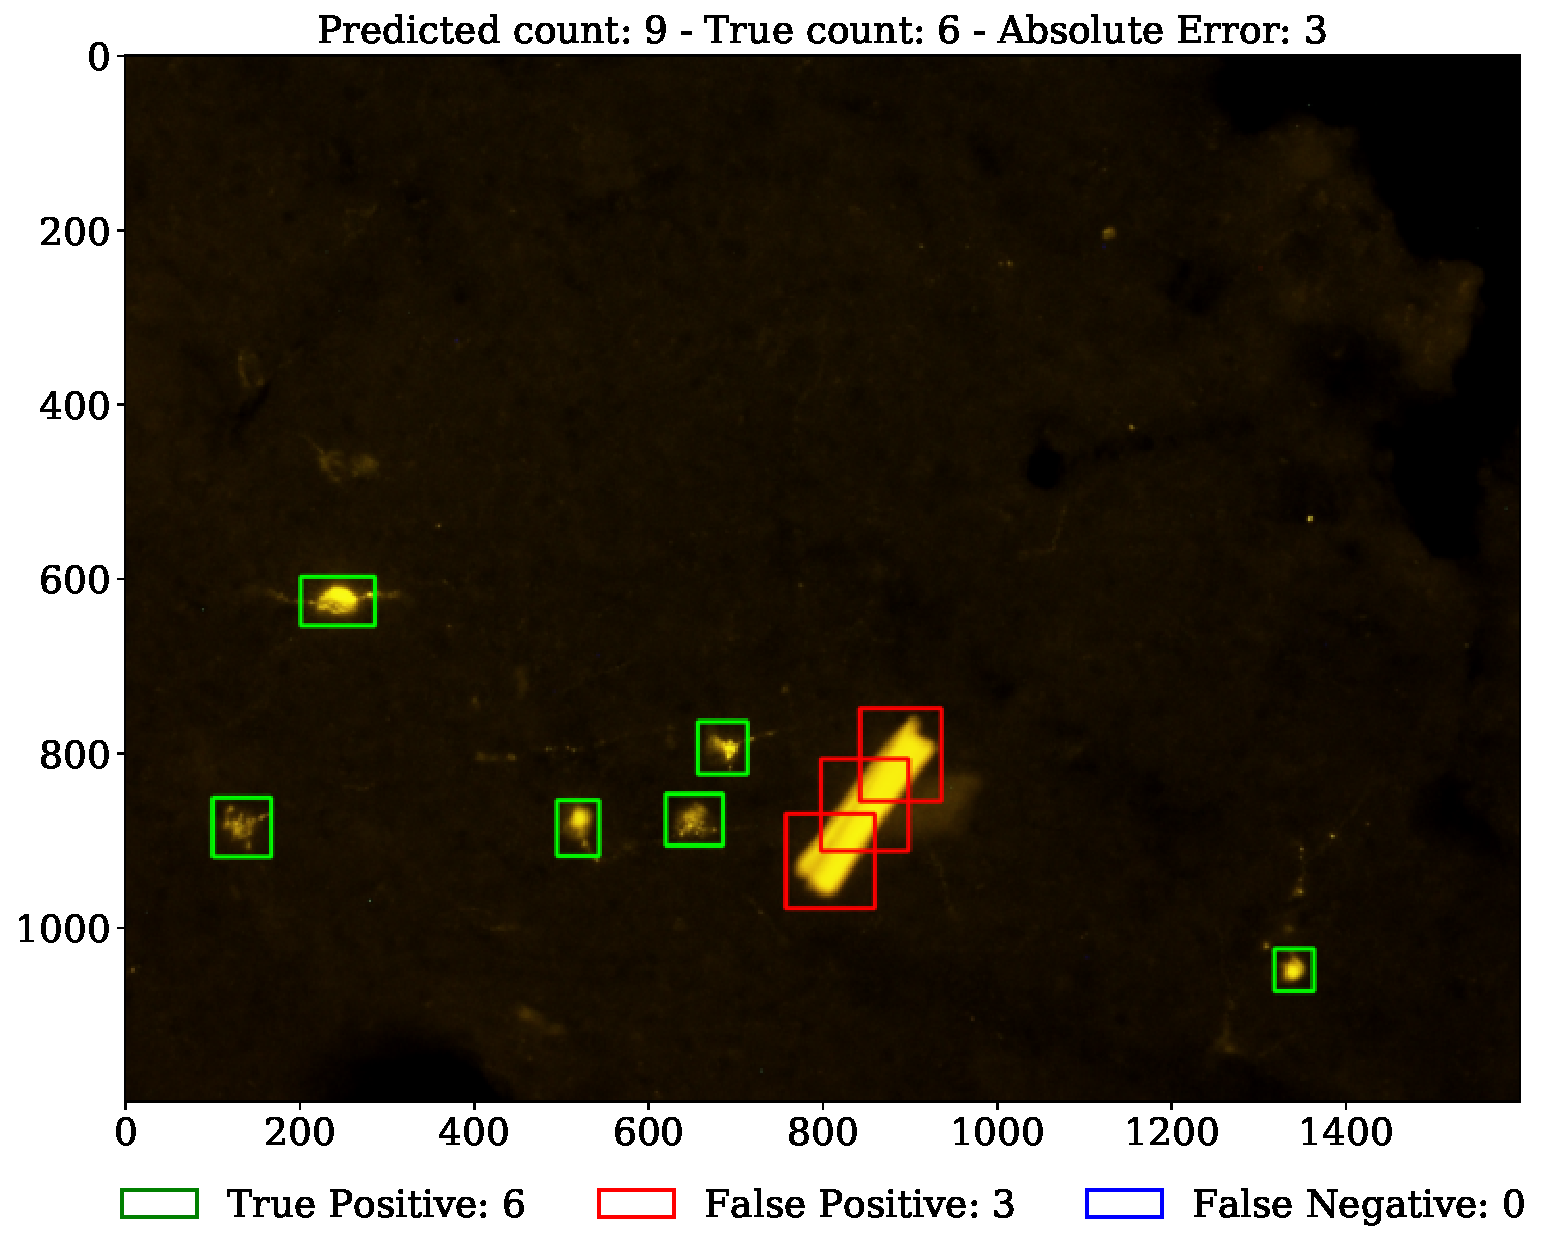
\includegraphics[width=\linewidth]{figures/140_results/pred_ResUnet:254.pdf}\label{fig:artifacts:clumping}
%     }
%     \caption{\textbf{Challenges and artifacts.}}
%     \label{fig:artifacts}
% \end{figure}%

% \begin{figure}[ht]\ContinuedFloat
%     \centering
%     \subfloat[\textit{Biological artifacts:} 
%     ]{
%     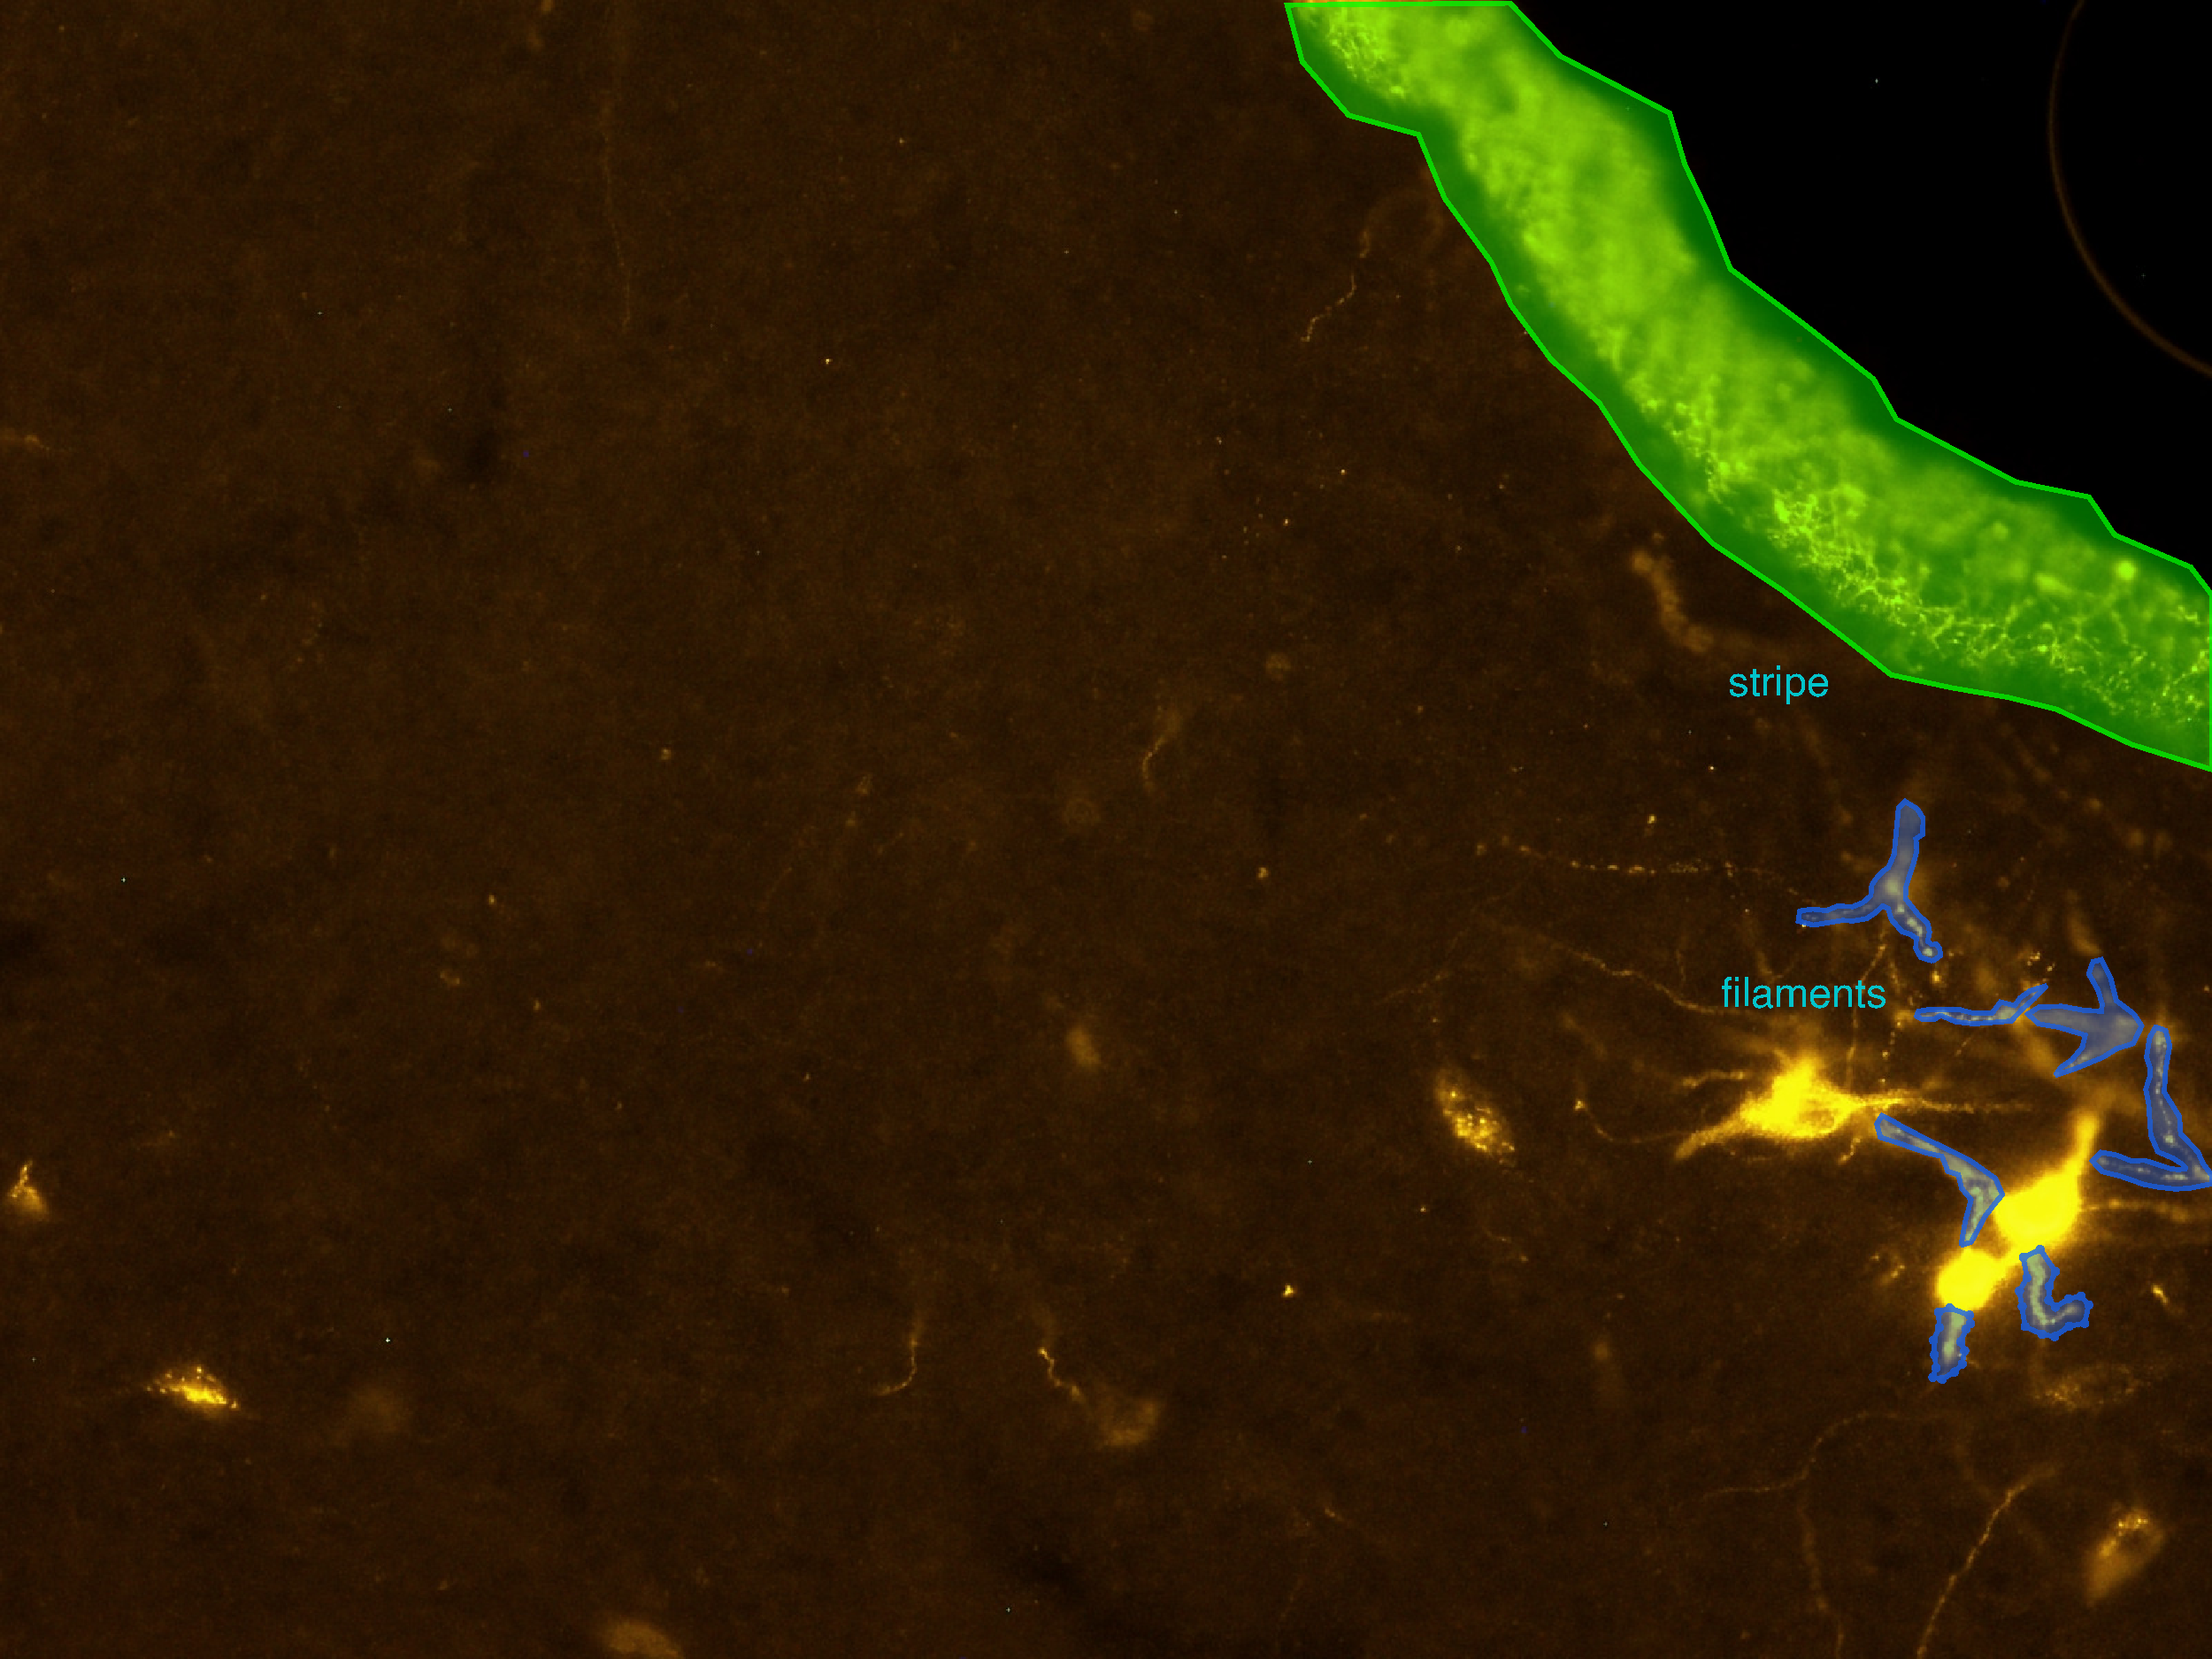
\includegraphics[width=\linewidth]{figures/120_dataset/challenges/stripe_and_filaments.pdf}\label{fig:artifacts:stripe}
%     }
%     \caption{\textbf{Challenges and artifacts. (2)}}
% \end{figure}%
% % \end{landscape}

% % \begin{landscape}
% \begin{figure}[ht]\ContinuedFloat
%     \centering
%     \subfloat[\textit{Technical artifacts:}
%     ]{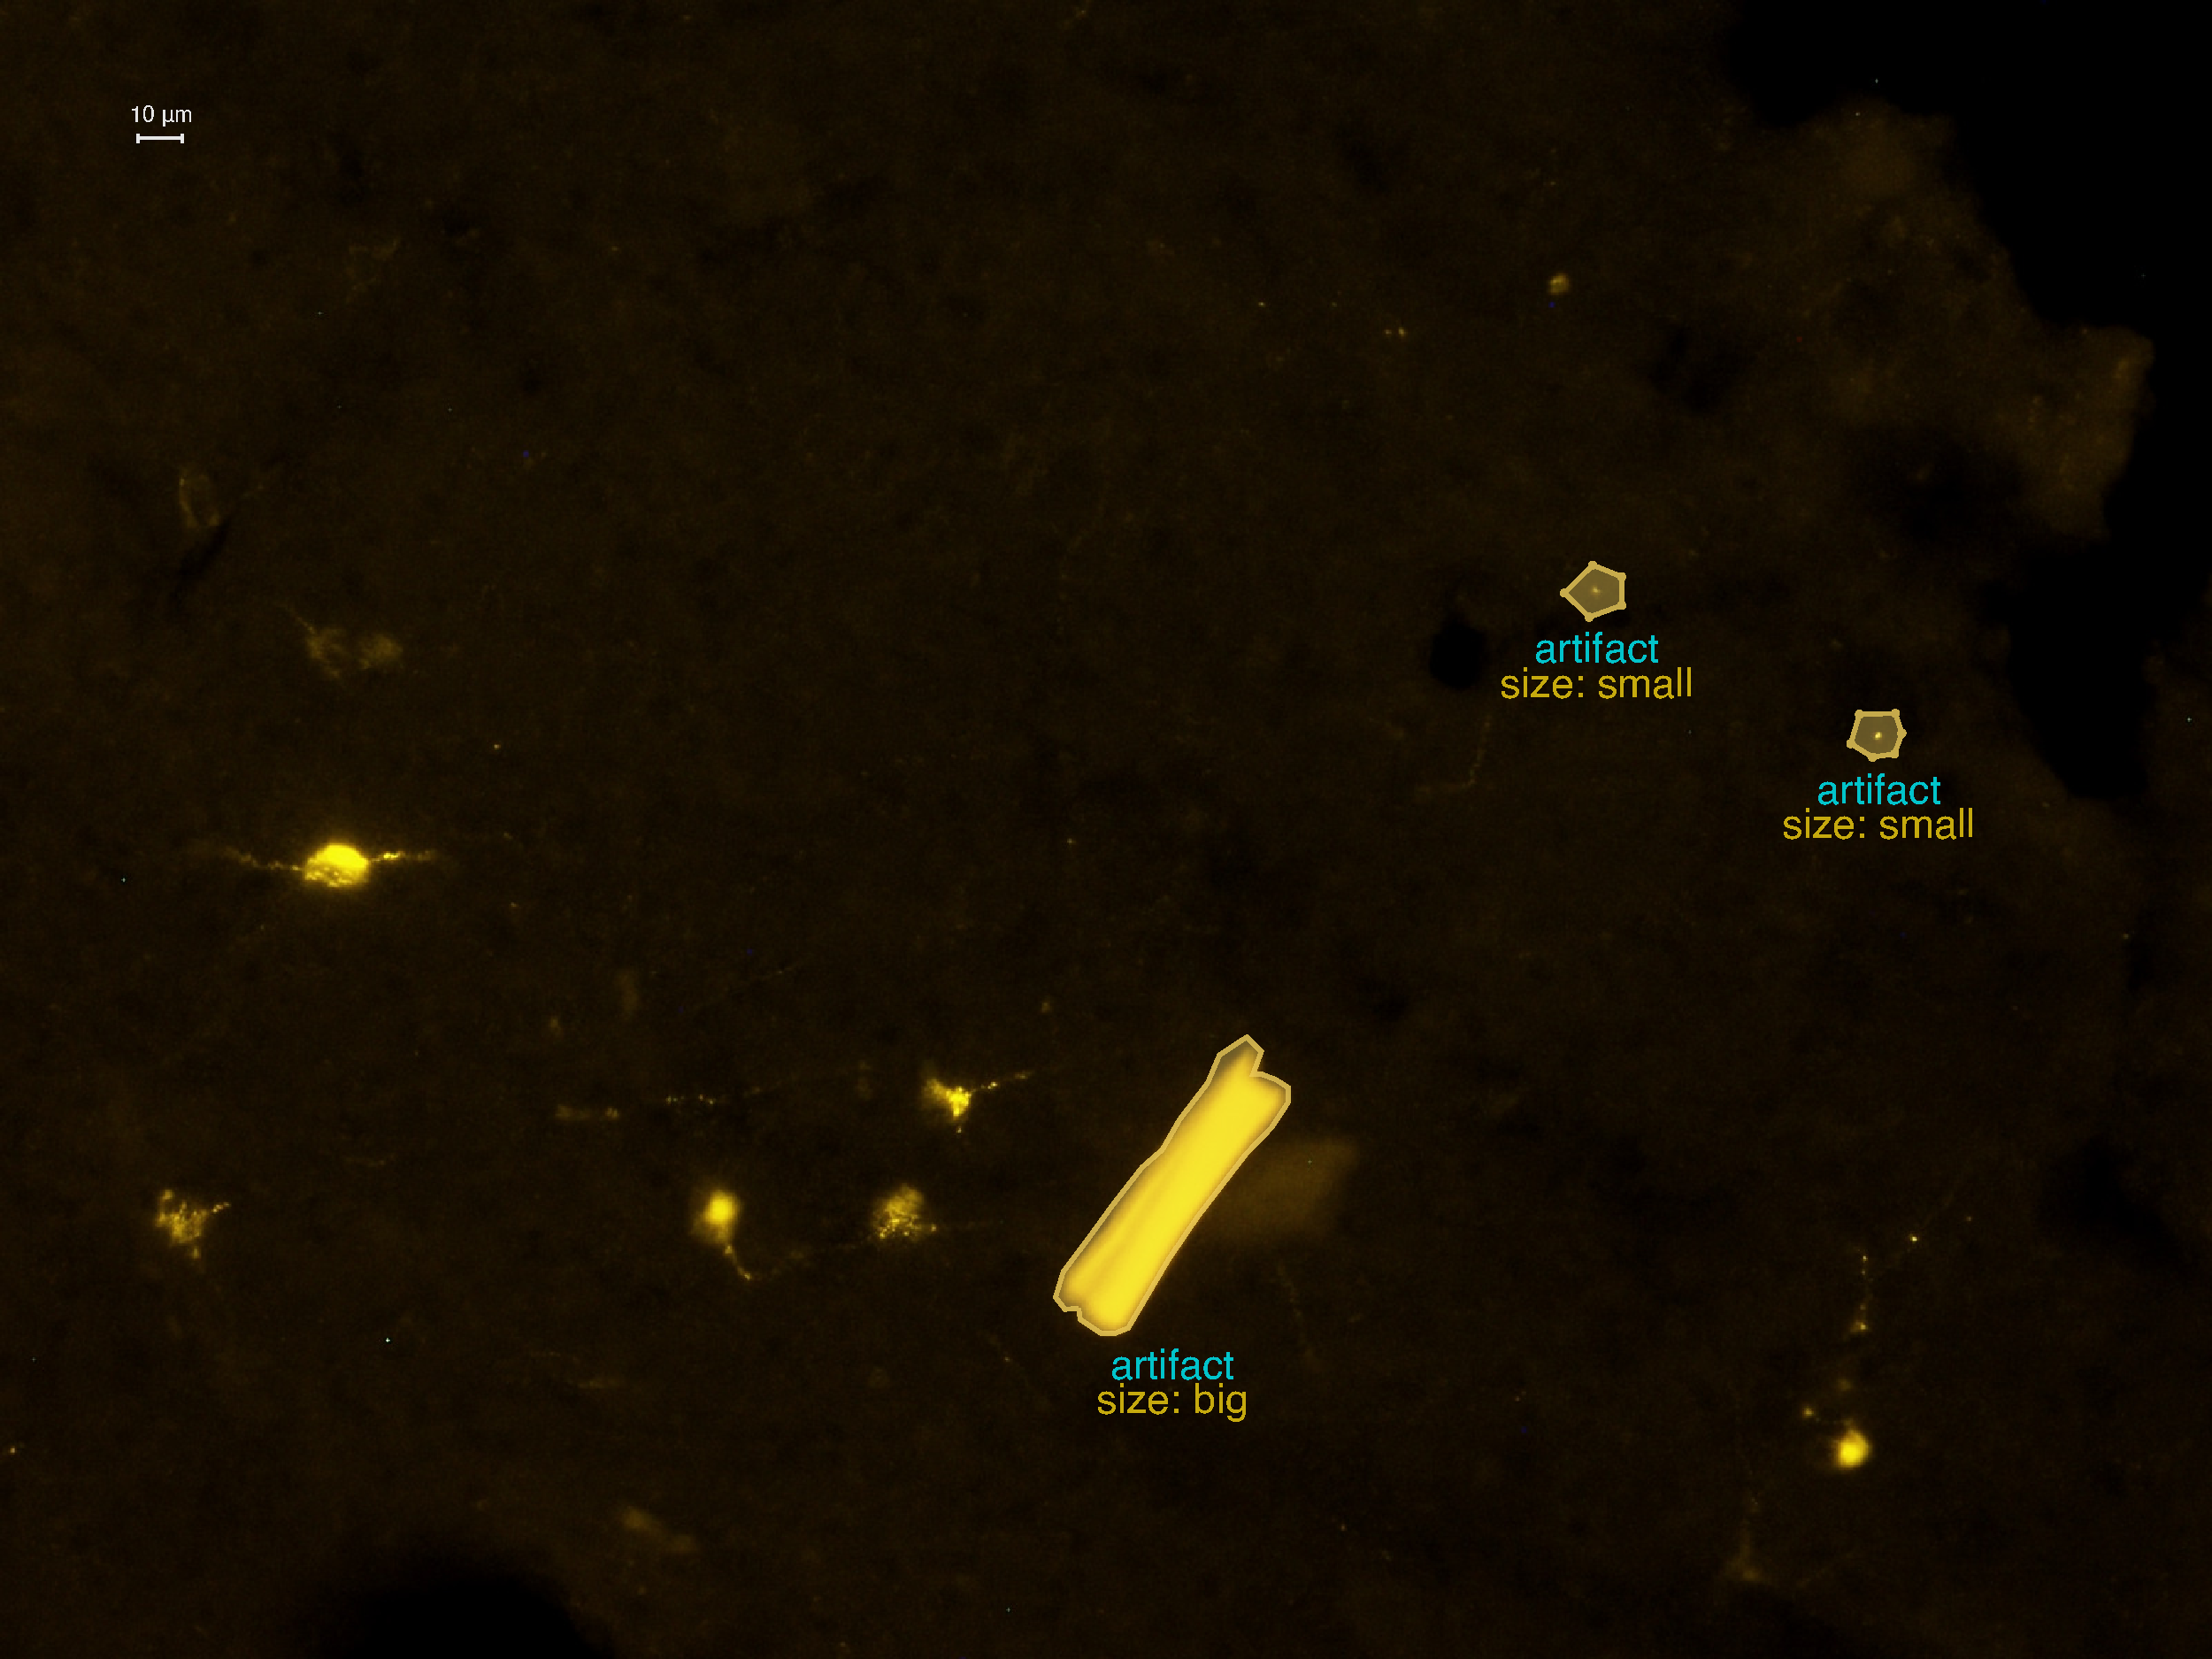
\includegraphics[width=\linewidth]{figures/120_dataset/challenges/artifacts.pdf}\label{fig:artifacts:macaroon}
%     }
%     \caption{\textbf{Challenges and artifacts. (3)}}
% \end{figure}
% \end{landscape}
% \clearpage
% \restoregeometry


% \savegeometry{origigeom}
% \clearpage
% \newgeometry{lmargin=1.5cm}
% \begin{landscape}

% \begin{figure}[!b]
% \centering
% \subfloat[]{
% 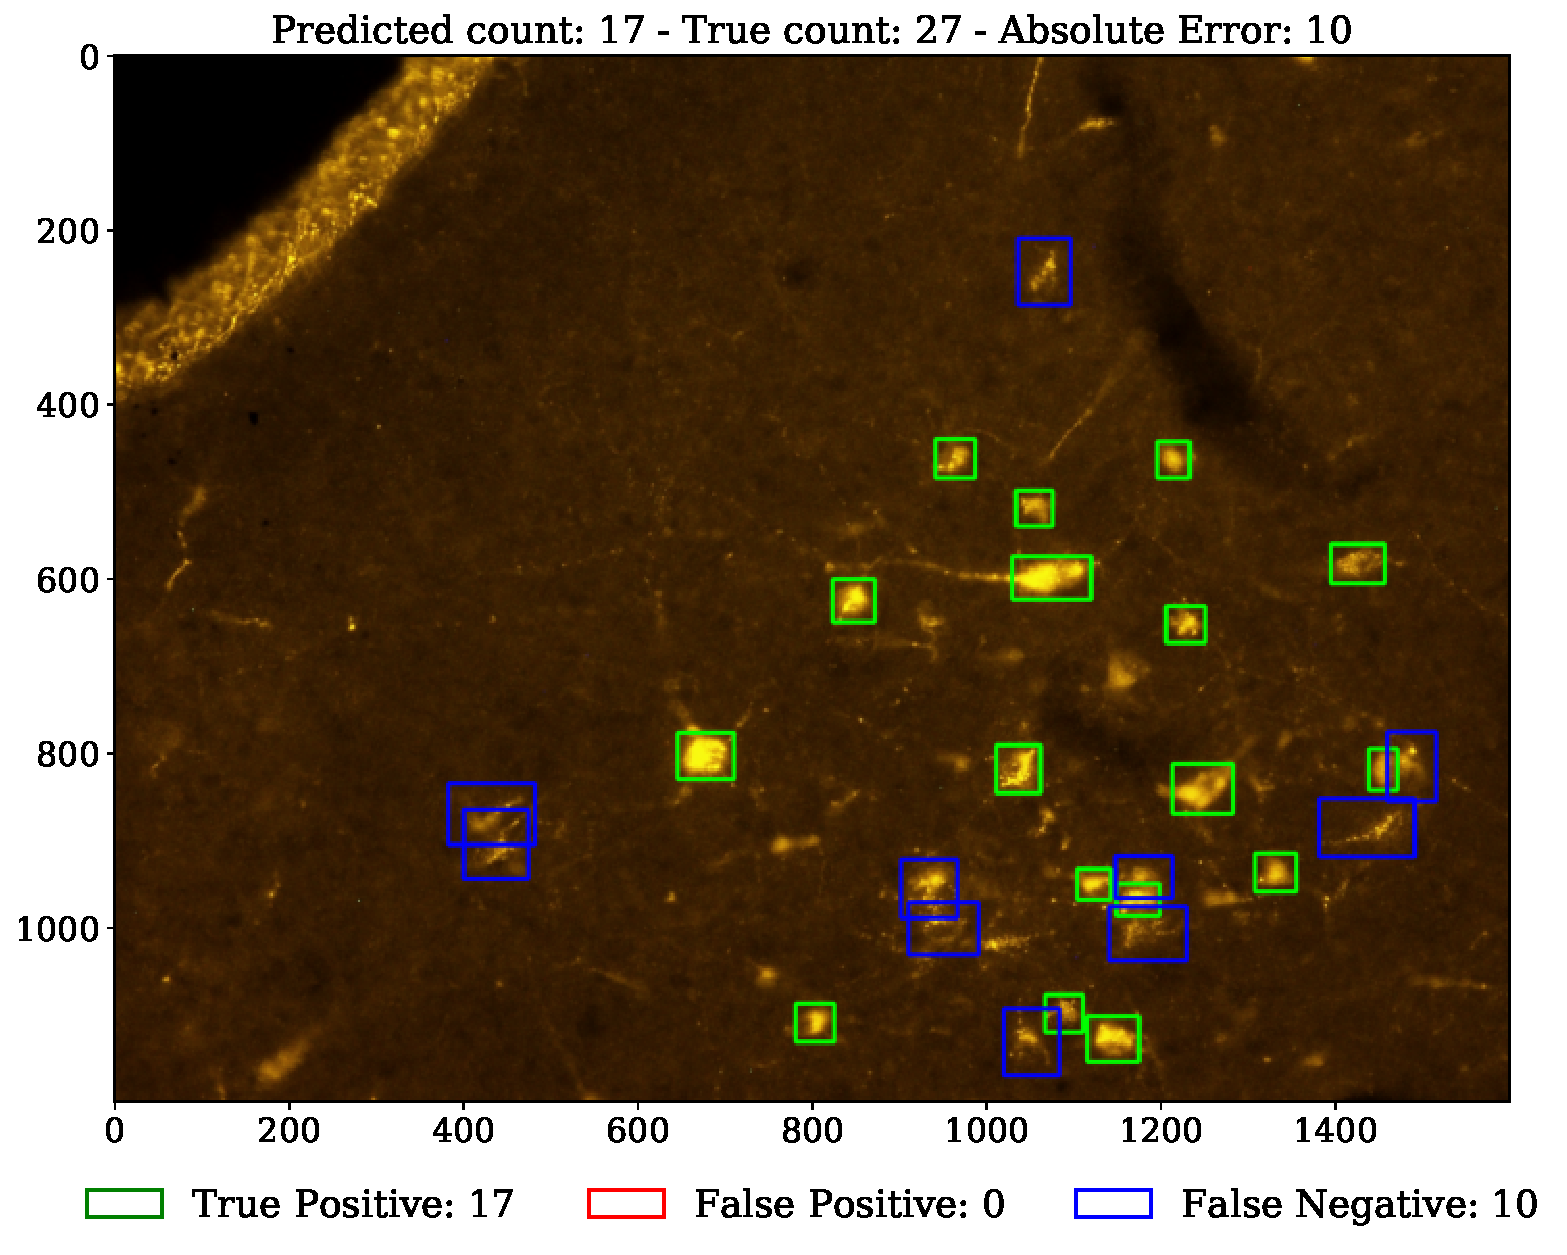
\includegraphics[width=\linewidth]{figures/140_results/pred_ResUnet_noAO:281.pdf}\label{fig:predictions:noAO}
% }
% \caption{\textbf{Results on test images}. 
% % Top row illustrates AO effect. 
% The c-ResUnet (no AO) correctly handles evident artifacts (\ref{fig:predictions:noAO}, top left corner), while the c-ResUnet fails with more problematic structures (\ref{fig:predictions:artifact}).
% % Bottom row highlights c-ResUnet predictive ability. 
% Notice how false positives (\ref{fig:predictions:false-positives}, red boxes) look like target cells. Likewise, the objects discarded (\ref{fig:predictions:false-negatives}, blue boxes) are similar to other stains that were not annotated.
% } 
% \label{fig:predictions}
% \end{figure}
% \begin{figure}[ht]\ContinuedFloat
% \centering

% \subfloat[]{
% 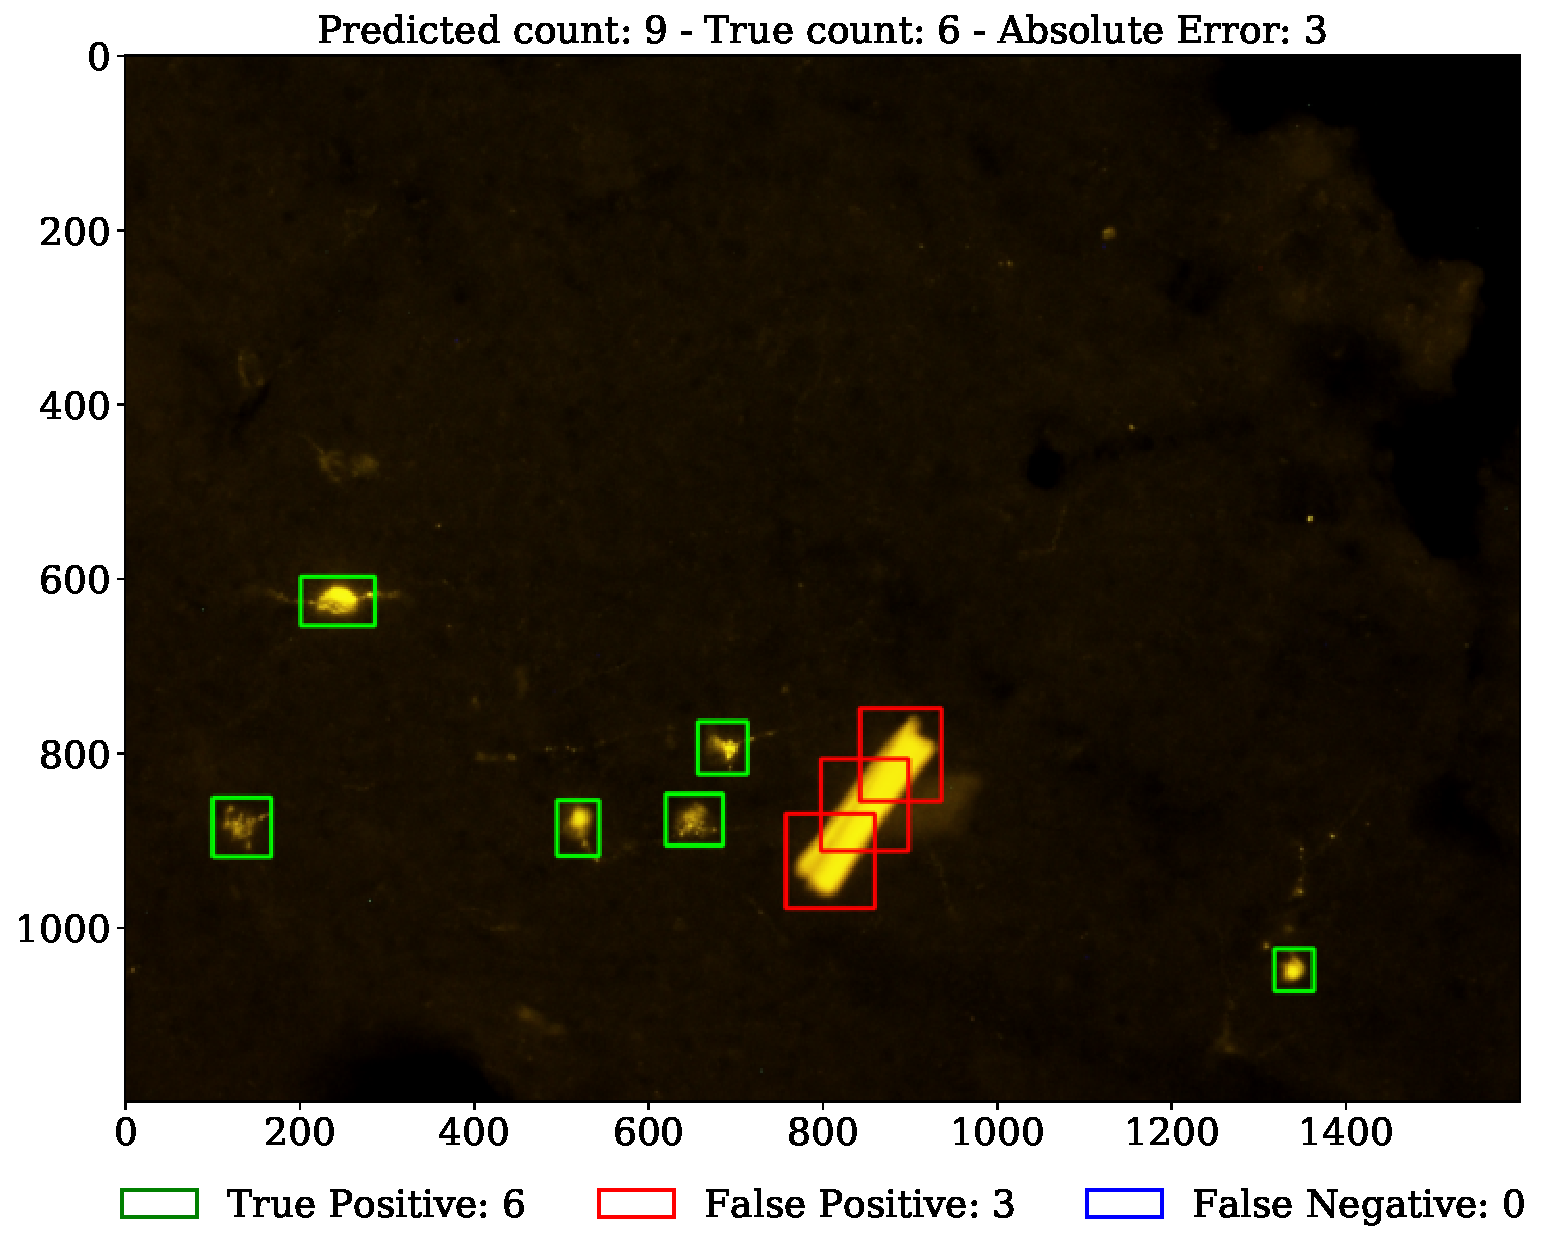
\includegraphics[width=\linewidth]{figures/140_results/pred_ResUnet:254.pdf}\label{fig:predictions:noAO}
% }
% \caption{\textbf{Results on test images}. 
% % Top row illustrates AO effect. 
% The c-ResUnet (no AO) correctly handles evident artifacts (\ref{fig:predictions:noAO}, top left corner), while the c-ResUnet fails with more problematic structures (\ref{fig:predictions:artifact}).
% % Bottom row highlights c-ResUnet predictive ability. 
% Notice how false positives (\ref{fig:predictions:false-positives}, red boxes) look like target cells. Likewise, the objects discarded (\ref{fig:predictions:false-negatives}, blue boxes) are similar to other stains that were not annotated.
% } 
% \label{fig:predictions}
% \end{figure}


% \begin{figure}[ht]\ContinuedFloat
% \centering
% \subfloat[]{
% 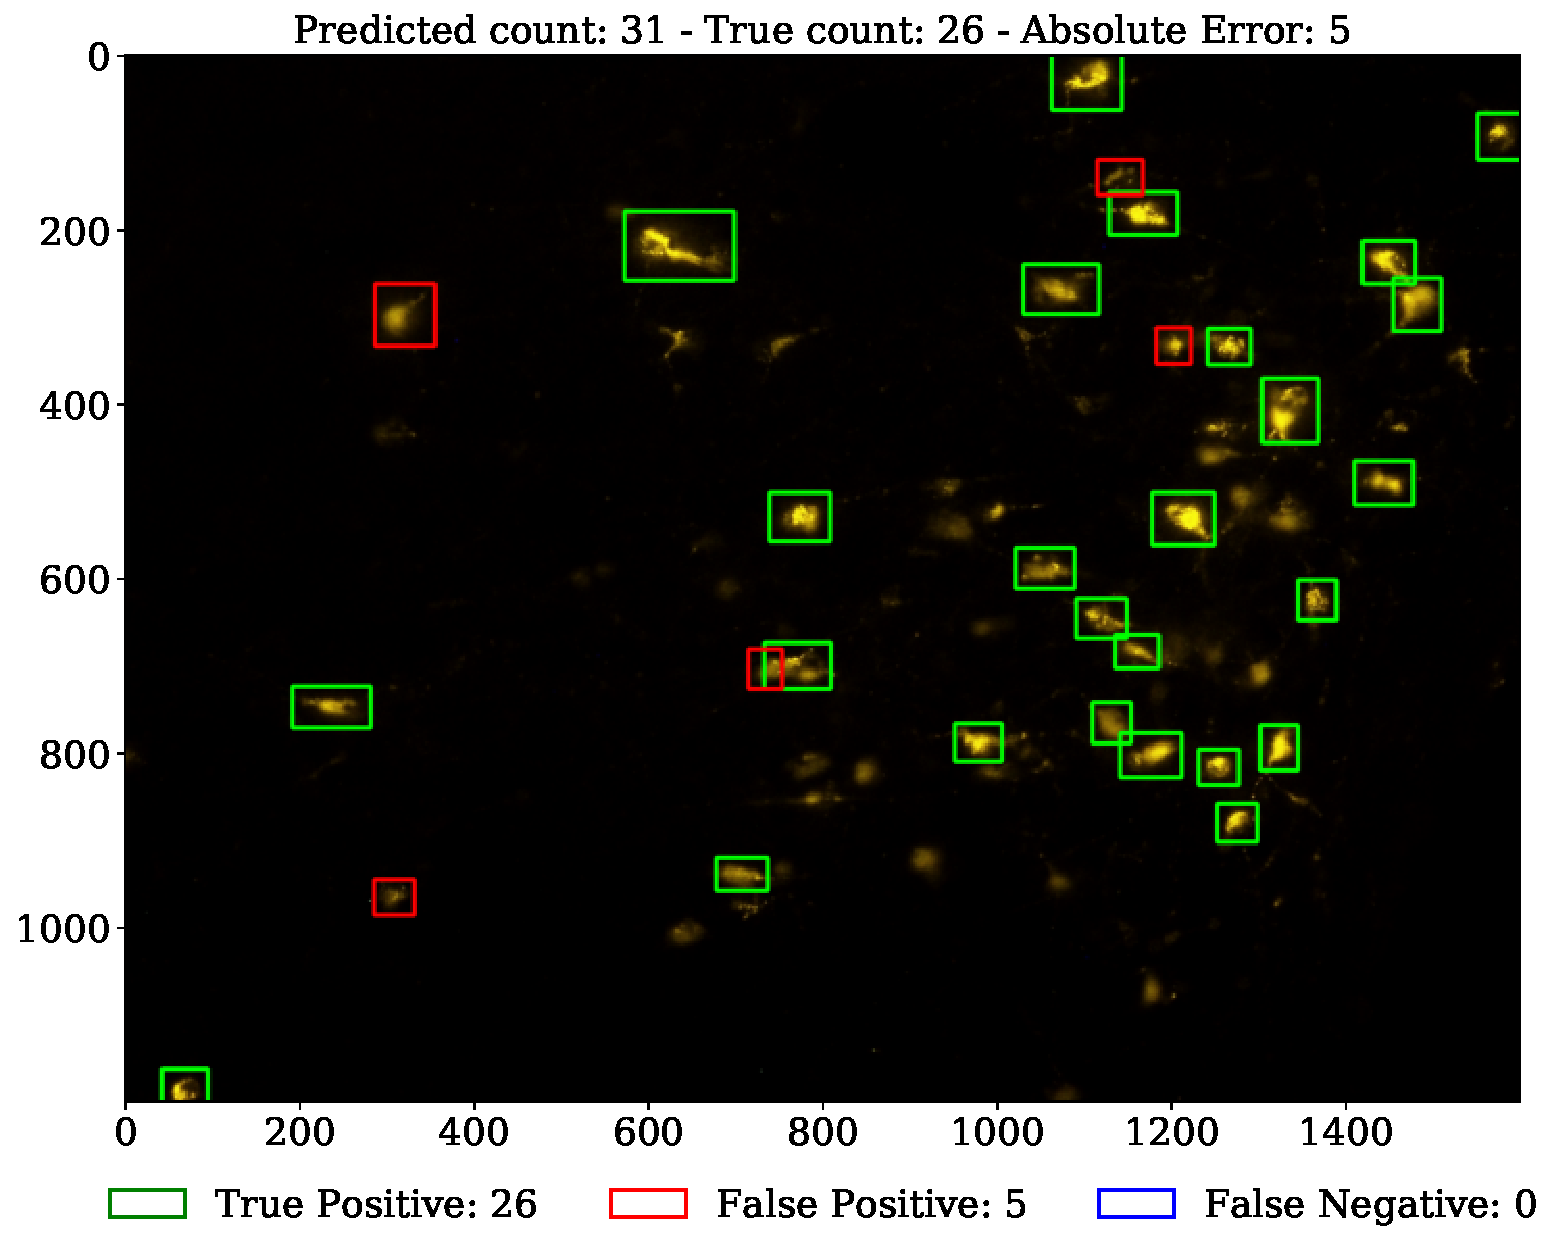
\includegraphics[width=\linewidth]{figures/140_results/pred_ResUnet:168.pdf}\label{fig:predictions:noAO}
% }
% \caption{\textbf{Results on test images}. 
% % Top row illustrates AO effect. 
% The c-ResUnet (no AO) correctly handles evident artifacts (\ref{fig:predictions:noAO}, top left corner), while the c-ResUnet fails with more problematic structures (\ref{fig:predictions:artifact}).
% % Bottom row highlights c-ResUnet predictive ability. 
% Notice how false positives (\ref{fig:predictions:false-positives}, red boxes) look like target cells. Likewise, the objects discarded (\ref{fig:predictions:false-negatives}, blue boxes) are similar to other stains that were not annotated.
% } 
% \label{fig:predictions}
% \end{figure}


% \begin{figure}[ht]\ContinuedFloat
% \centering
% \subfloat[]{
% 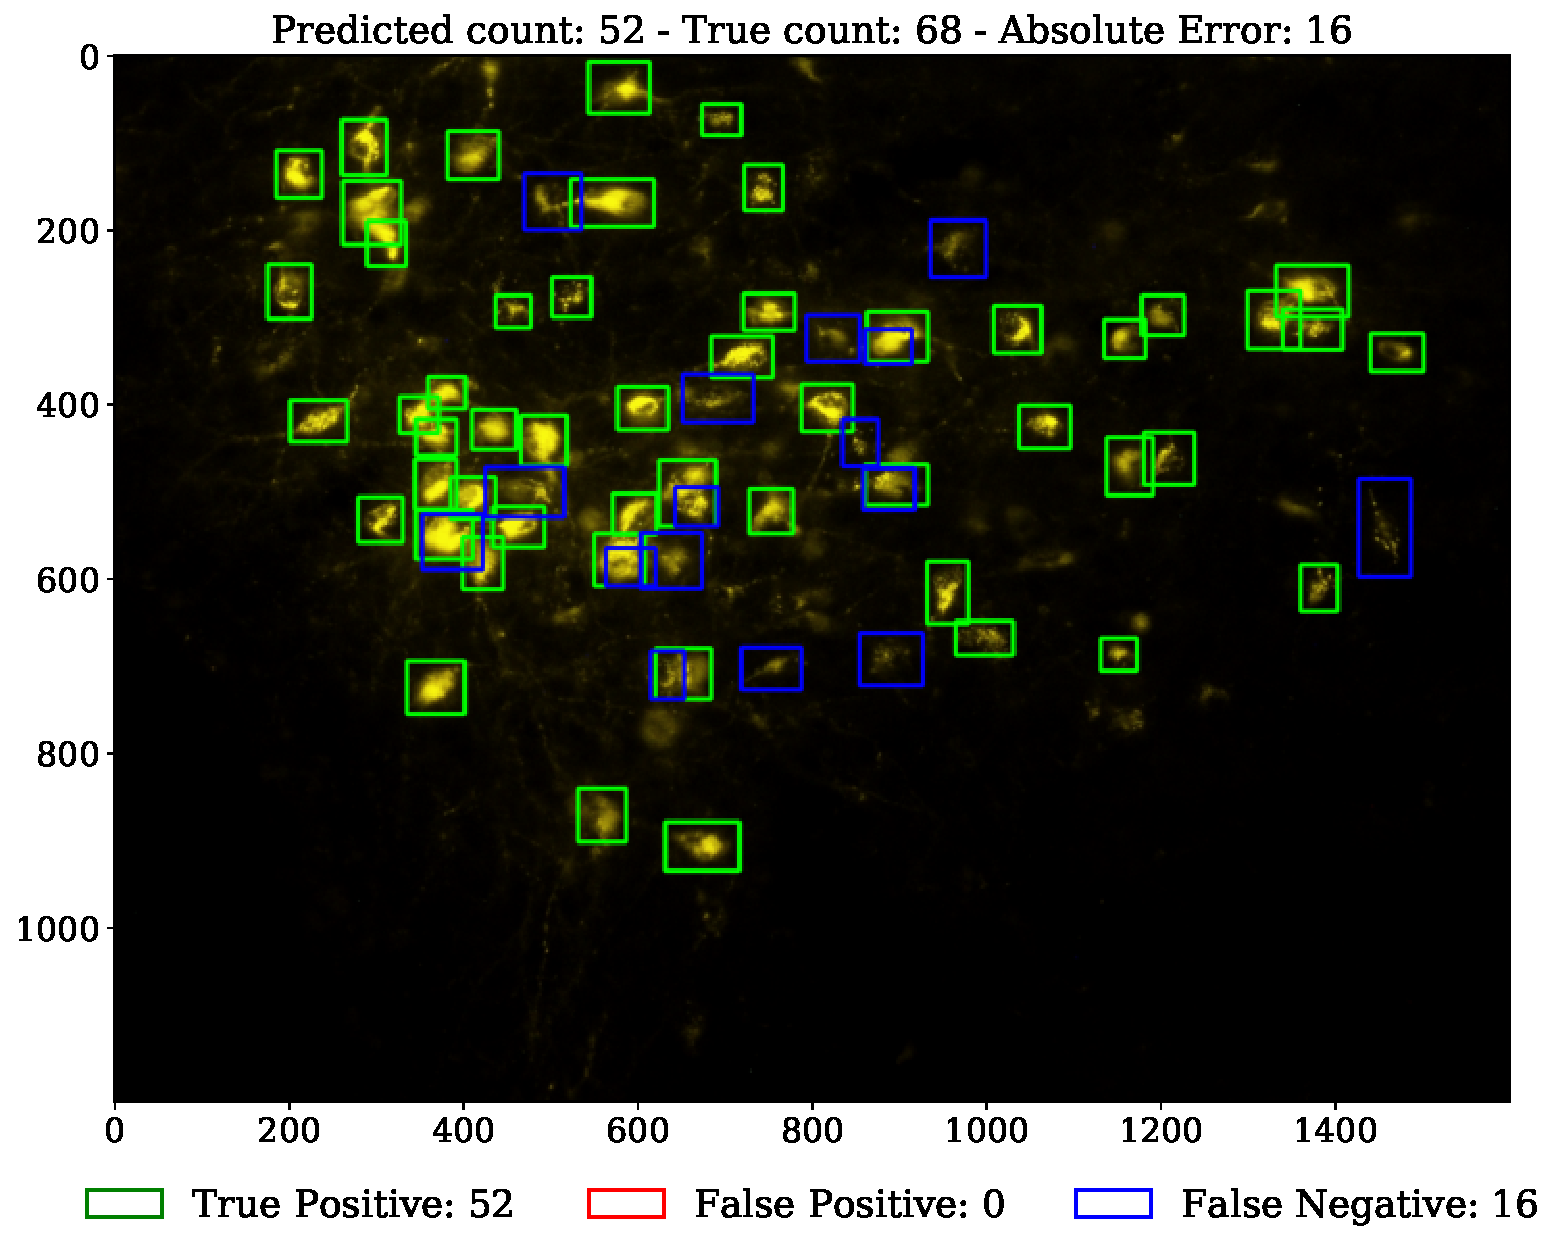
\includegraphics[width=\linewidth]{figures/140_results/pred_ResUnet:278.pdf}\label{fig:predictions:noAO}
% }
% \caption{\textbf{Results on test images}. 
% % Top row illustrates AO effect. 
% The c-ResUnet (no AO) correctly handles evident artifacts (\ref{fig:predictions:noAO}, top left corner), while the c-ResUnet fails with more problematic structures (\ref{fig:predictions:artifact}).
% % Bottom row highlights c-ResUnet predictive ability. 
% Notice how false positives (\ref{fig:predictions:false-positives}, red boxes) look like target cells. Likewise, the objects discarded (\ref{fig:predictions:false-negatives}, blue boxes) are similar to other stains that were not annotated.
% } 
% \label{fig:predictions}
% \end{figure}

% \end{landscape}

% \clearpage
% \restoregeometry




\begin{figure}[!b]
\centering
\subfloat[stripes and filaments]{
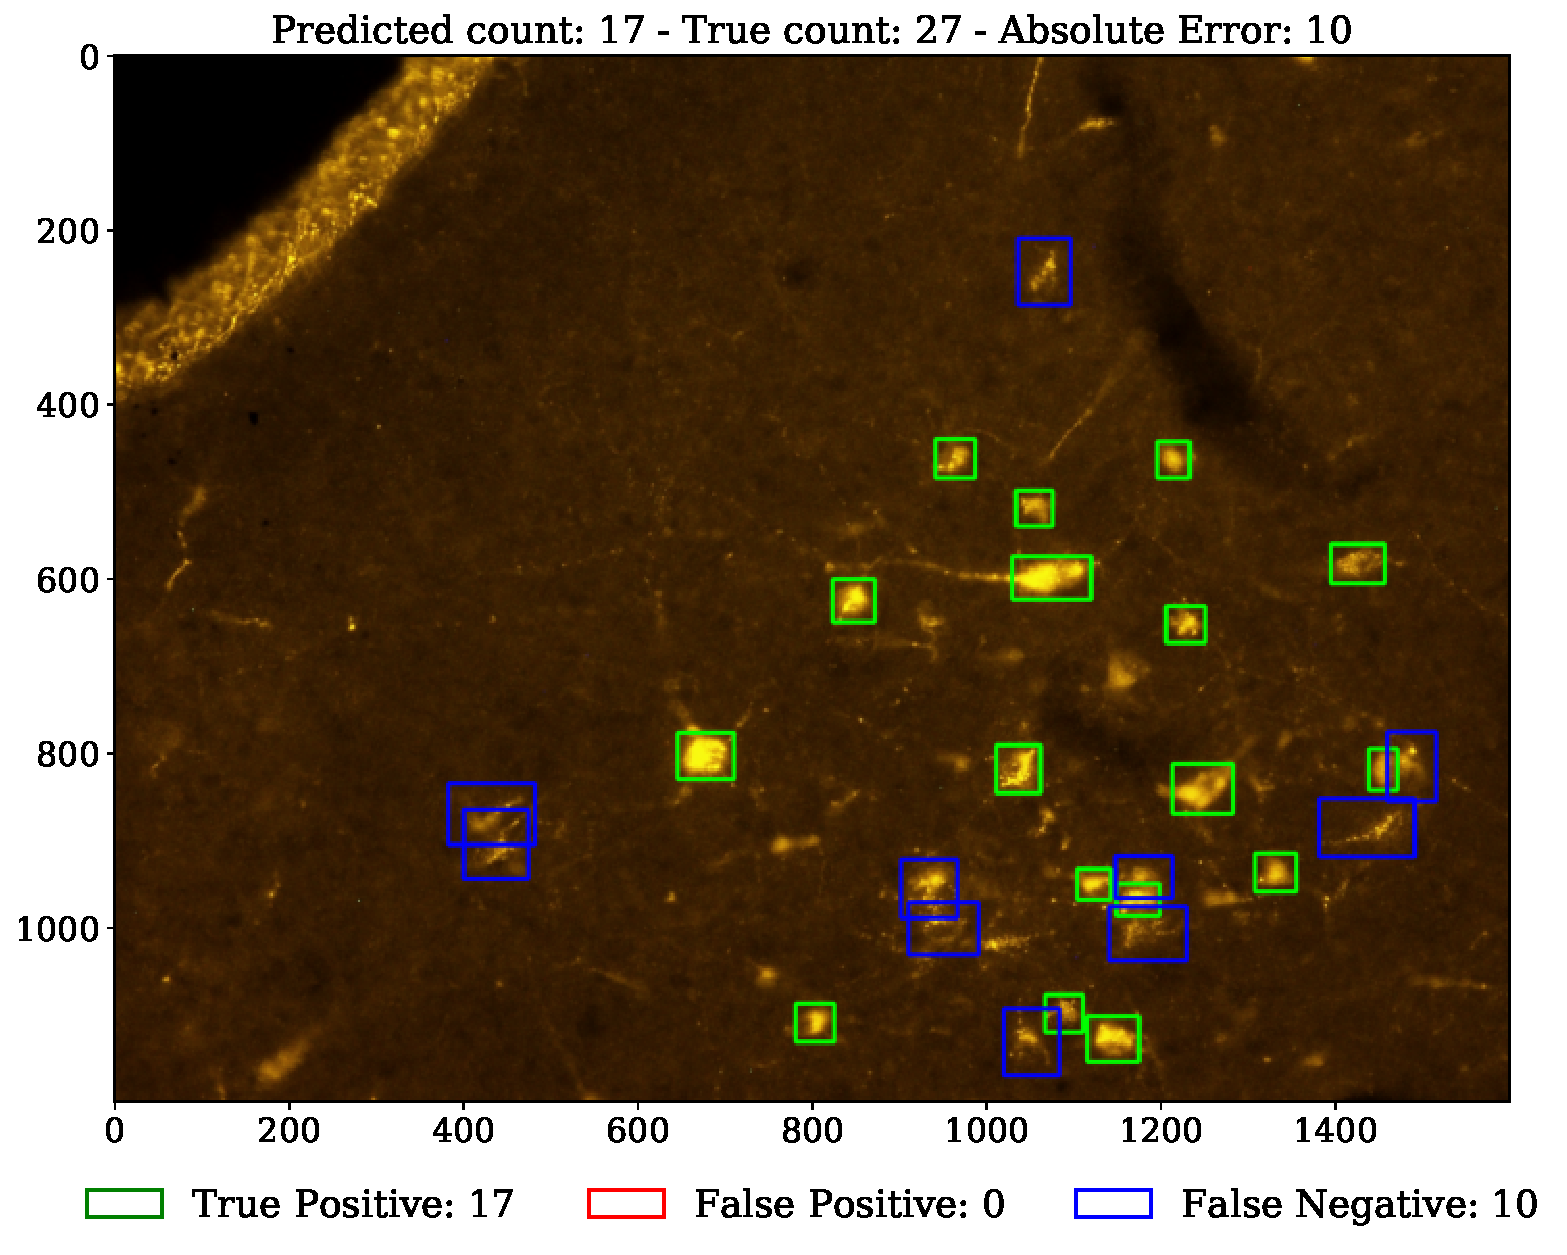
\includegraphics[width=\textwidth]{figures/140_results/pred_ResUnet_noAO:281.pdf}\label{fig:predictions:noAO}
}
\caption{\textbf{Results on test images.} 
The c-ResUnet (no AO) correctly handles the evident stripe in the top left corner despite not receiving dedicated oversampling for such biological structures.
% Filaments are also correctly interpreted
} 
\label{fig:predictions}
\end{figure}
\begin{figure}[ht]\ContinuedFloat
\centering

\subfloat[technical artifacts]{
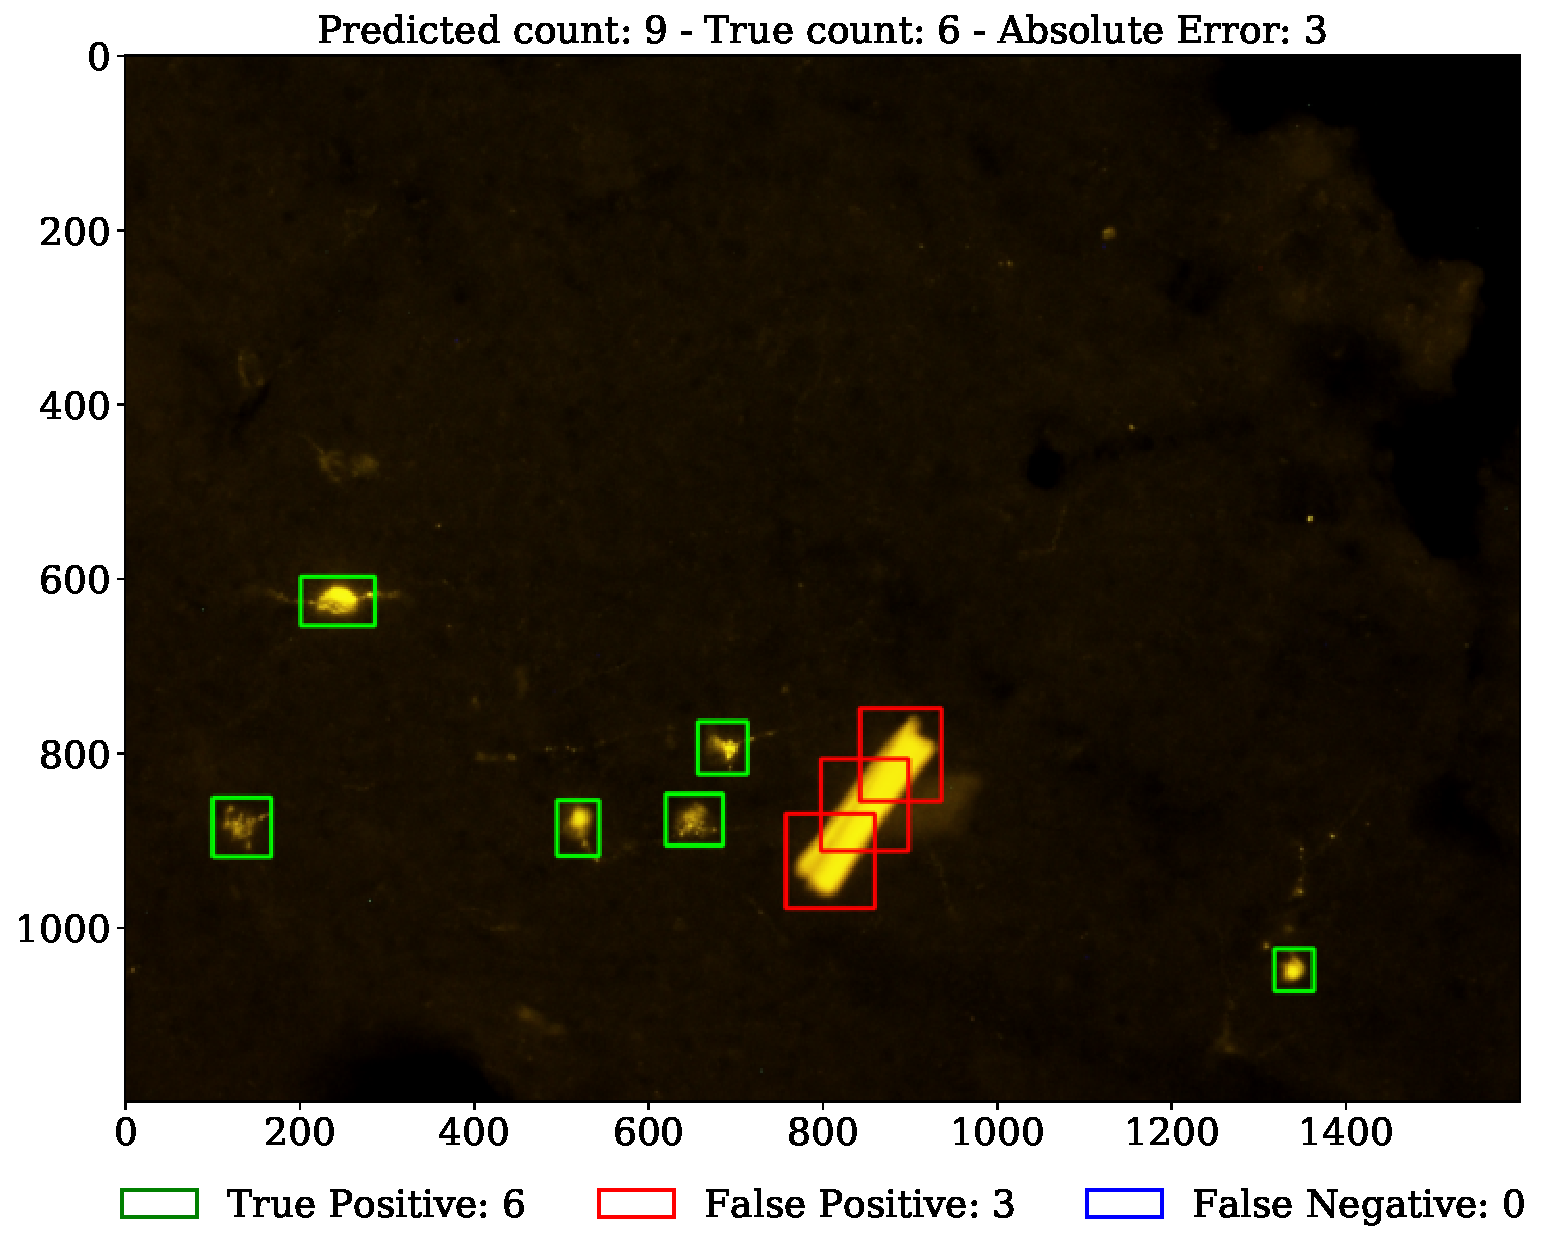
\includegraphics[width=\textwidth]{figures/140_results/pred_ResUnet:254.pdf}\label{fig:predictions:artifact}
}
\caption{\textbf{Results on test images (2).} 
The c-ResUnet fails with the \mbox{macaroni-shaped} artifact in the middle of the picture, suggesting that the oversampling strategy is not effective in this case. However, notice that no other similar artifacts are present in the training set.
} 
\end{figure}


\begin{figure}[ht]\ContinuedFloat
\centering
\subfloat[false positives]{
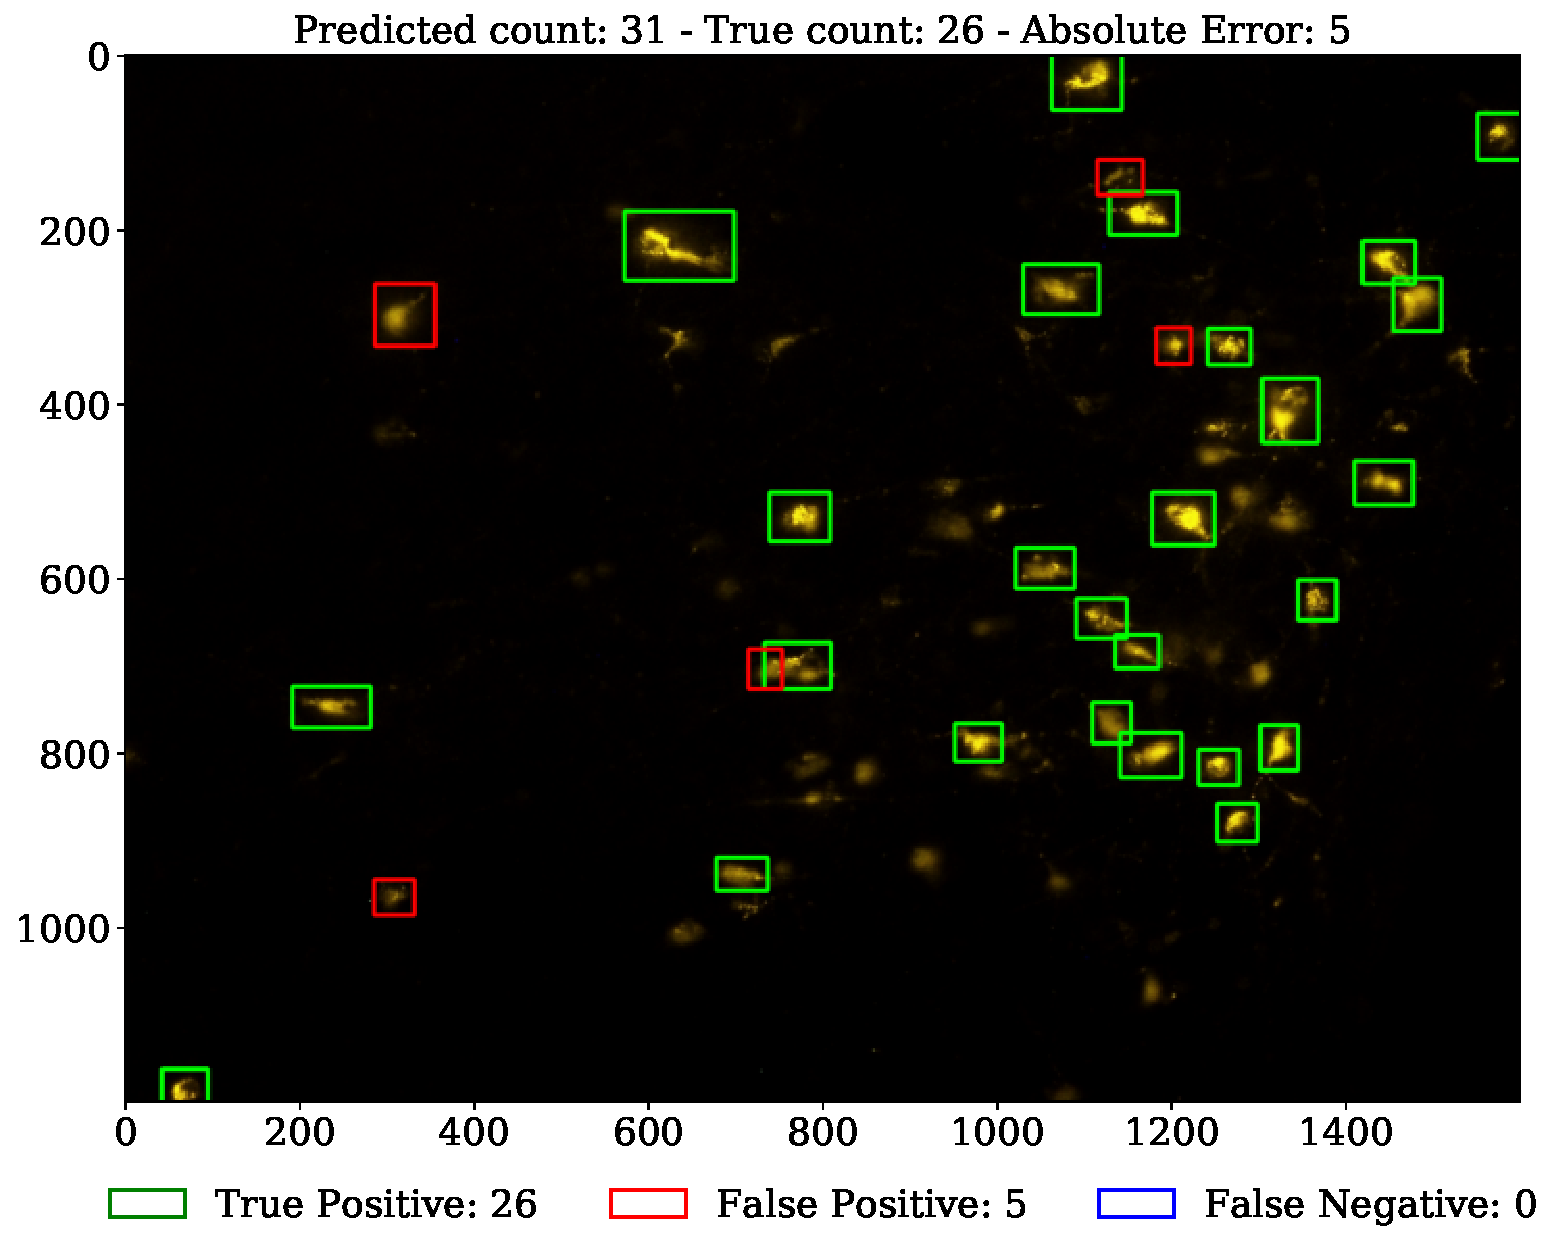
\includegraphics[width=\textwidth]{figures/140_results/pred_ResUnet:168.pdf}\label{fig:predictions:false-positives}
}
\caption{\textbf{Results on test images (3).} 
The c-ResUnet sometimes produces false positives (red boxes), i.e. it labels as cell structures that are not annotated by the researcher.
However, the difference with marked cells is marginal (cf. also with \hyperref[fig:predictions:false-negatives]{d}), suggesting that these errors may lie within the limits of arbitrariness intrinsic to the task.
} 
\end{figure}


\begin{figure}[ht]\ContinuedFloat
\centering
\subfloat[false negatives]{
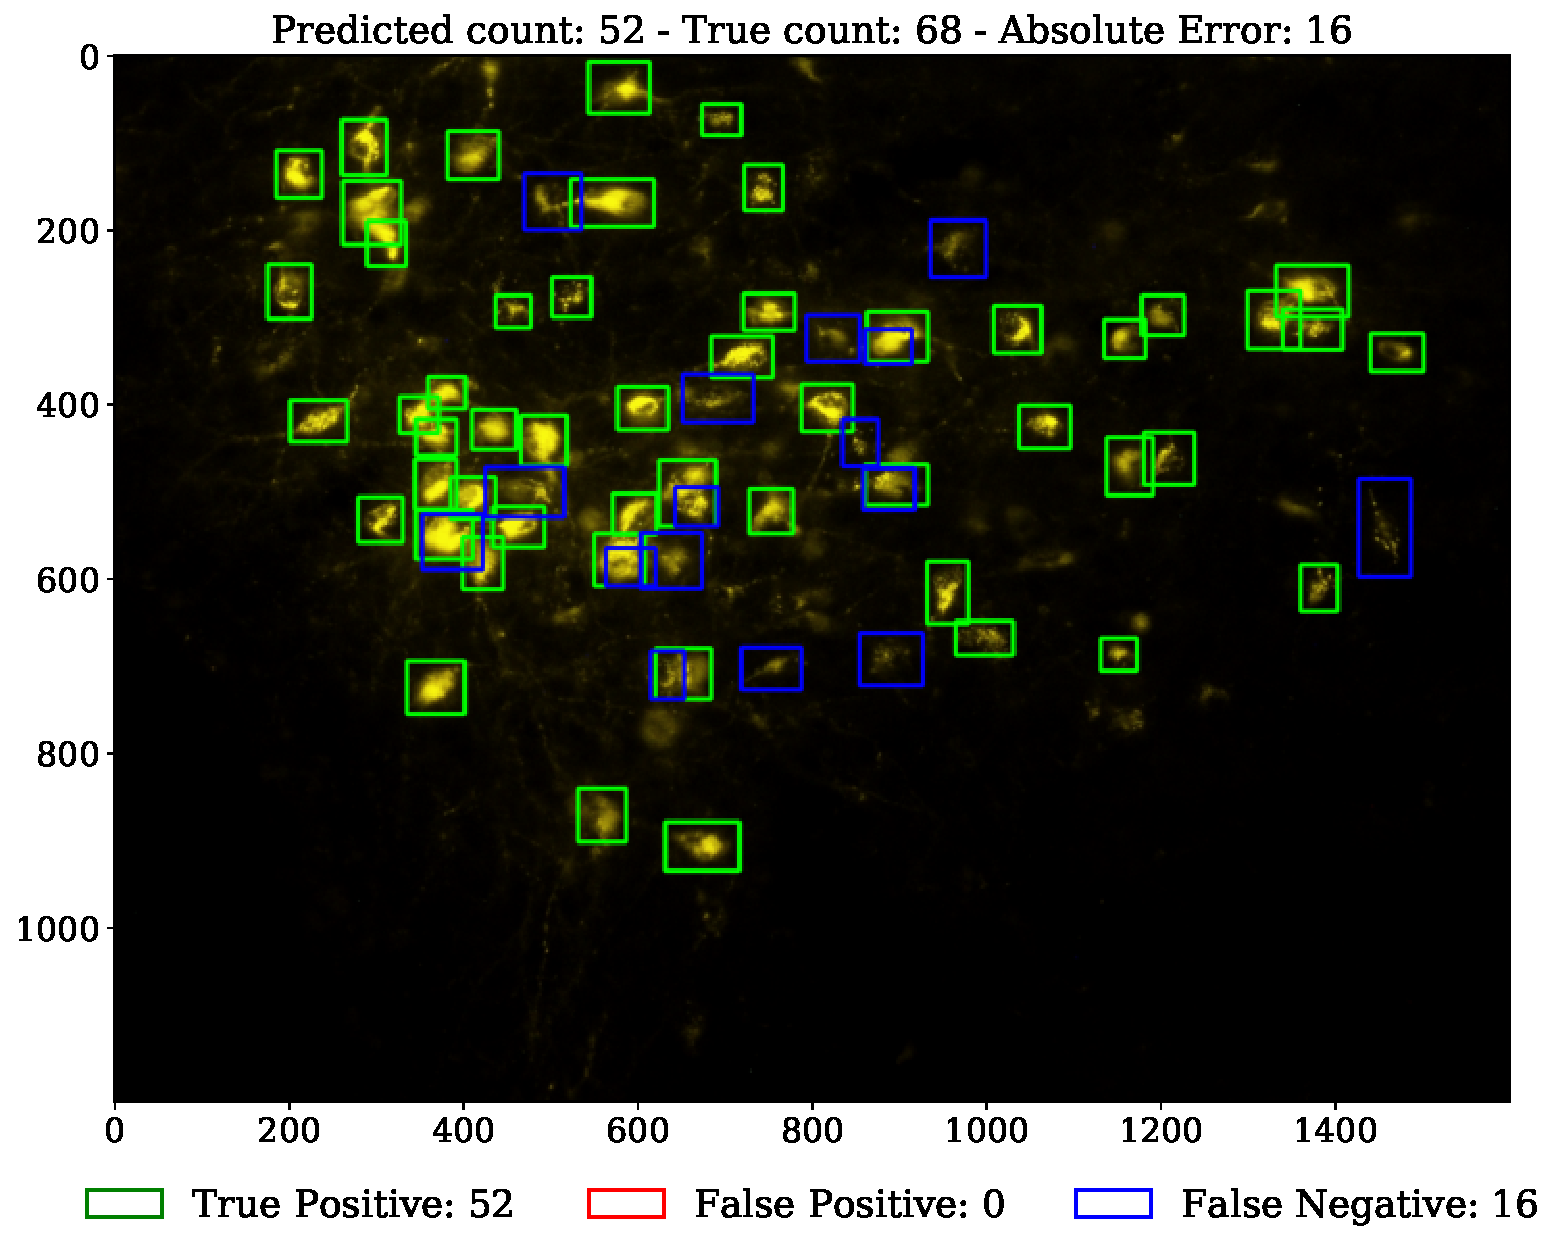
\includegraphics[width=\textwidth]{figures/140_results/pred_ResUnet:278.pdf}\label{fig:predictions:false-negatives}
}
\caption{\textbf{Results on test images (4).}
% Top row illustrates AO effect. 
The c-ResUnet is generally conservative in predictions, thus generating false positives (blue boxes).
However, these are similar to other stains that were not annotated (cf. also with \hyperref[fig:predictions:false-positives]{c}), thus falling again within the limits of operator's interpretation.
} 
\end{figure}









% \savegeometry{origigeom}
% \clearpage
% \newgeometry{lmargin=1.5cm}


% \begin{figure}[!b]
% \centering
% \subfloat[]{
% 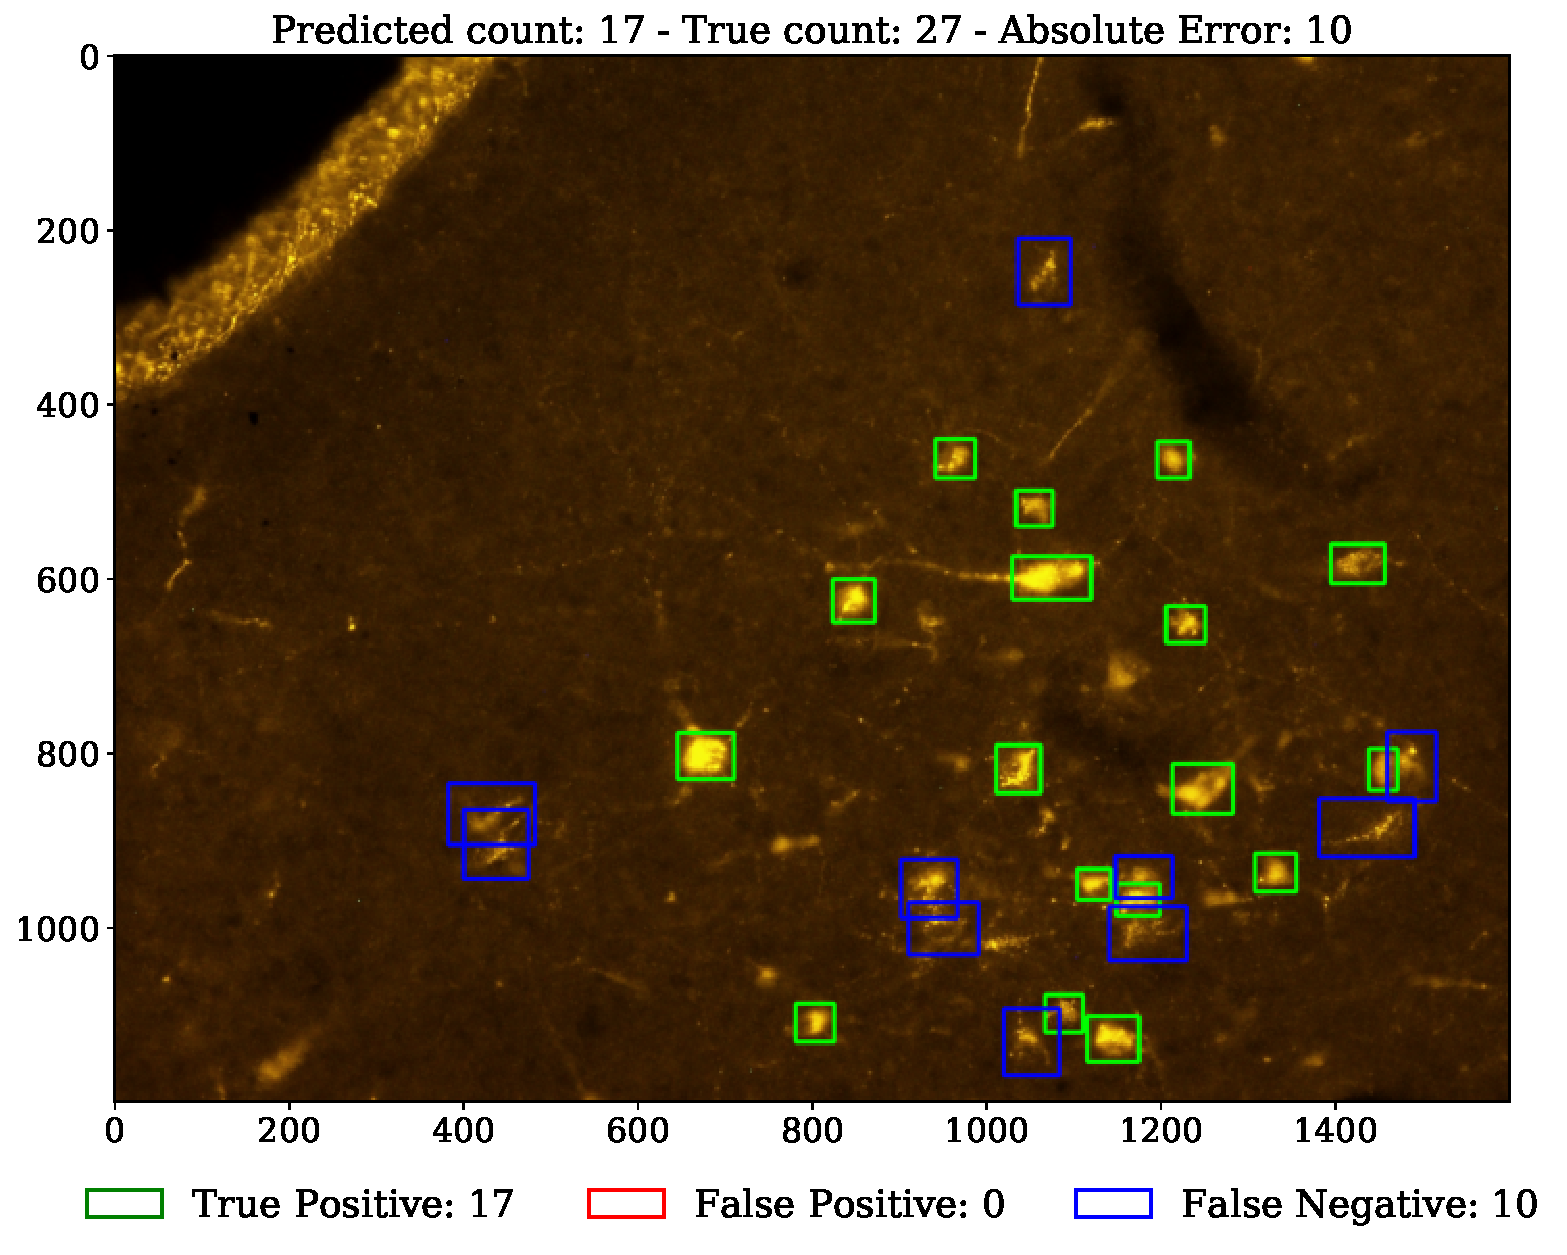
\includegraphics[width=\textwidth]{figures/140_results/pred_ResUnet_noAO:281.pdf}\label{fig:predictions:noAO}
% }
% \caption{\textbf{Results on test images}. 
% % Top row illustrates AO effect. 
% The c-ResUnet (no AO) correctly handles evident artifacts (\ref{fig:predictions:noAO}, top left corner), while the c-ResUnet fails with more problematic structures (\ref{fig:predictions:artifact}).
% % Bottom row highlights c-ResUnet predictive ability. 
% Notice how false positives (\ref{fig:predictions:false-positives}, red boxes) look like target cells. Likewise, the objects discarded (\ref{fig:predictions:false-negatives}, blue boxes) are similar to other stains that were not annotated.
% } 
% \label{fig:predictions}
% \end{figure}
% \begin{figure}[ht]\ContinuedFloat
% \centering

% \subfloat[]{
% 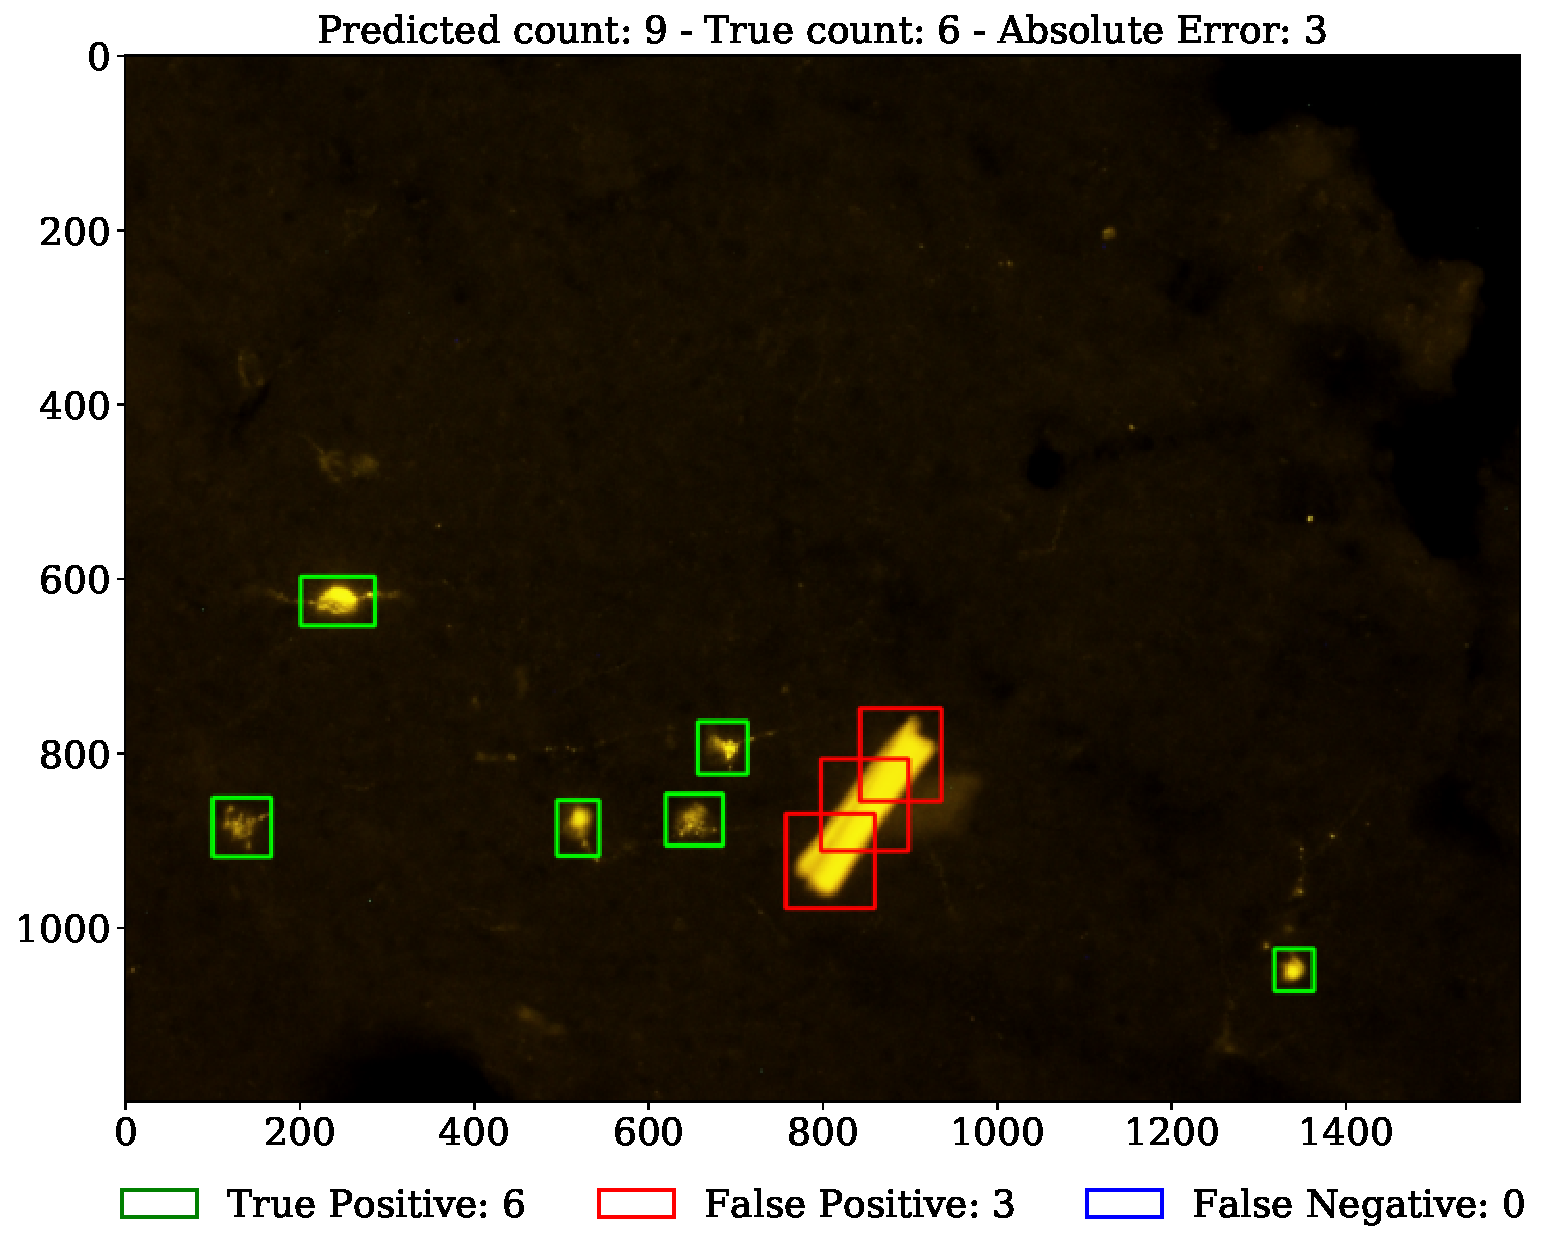
\includegraphics[width=\textwidth]{figures/140_results/pred_ResUnet:254.pdf}\label{fig:predictions:noAO}
% }
% \caption{\textbf{Results on test images}. 
% % Top row illustrates AO effect. 
% The c-ResUnet (no AO) correctly handles evident artifacts (\ref{fig:predictions:noAO}, top left corner), while the c-ResUnet fails with more problematic structures (\ref{fig:predictions:artifact}).
% % Bottom row highlights c-ResUnet predictive ability. 
% Notice how false positives (\ref{fig:predictions:false-positives}, red boxes) look like target cells. Likewise, the objects discarded (\ref{fig:predictions:false-negatives}, blue boxes) are similar to other stains that were not annotated.
% } 
% \label{fig:predictions}
% \end{figure}


% \begin{figure}[ht]\ContinuedFloat
% \centering
% \subfloat[]{
% 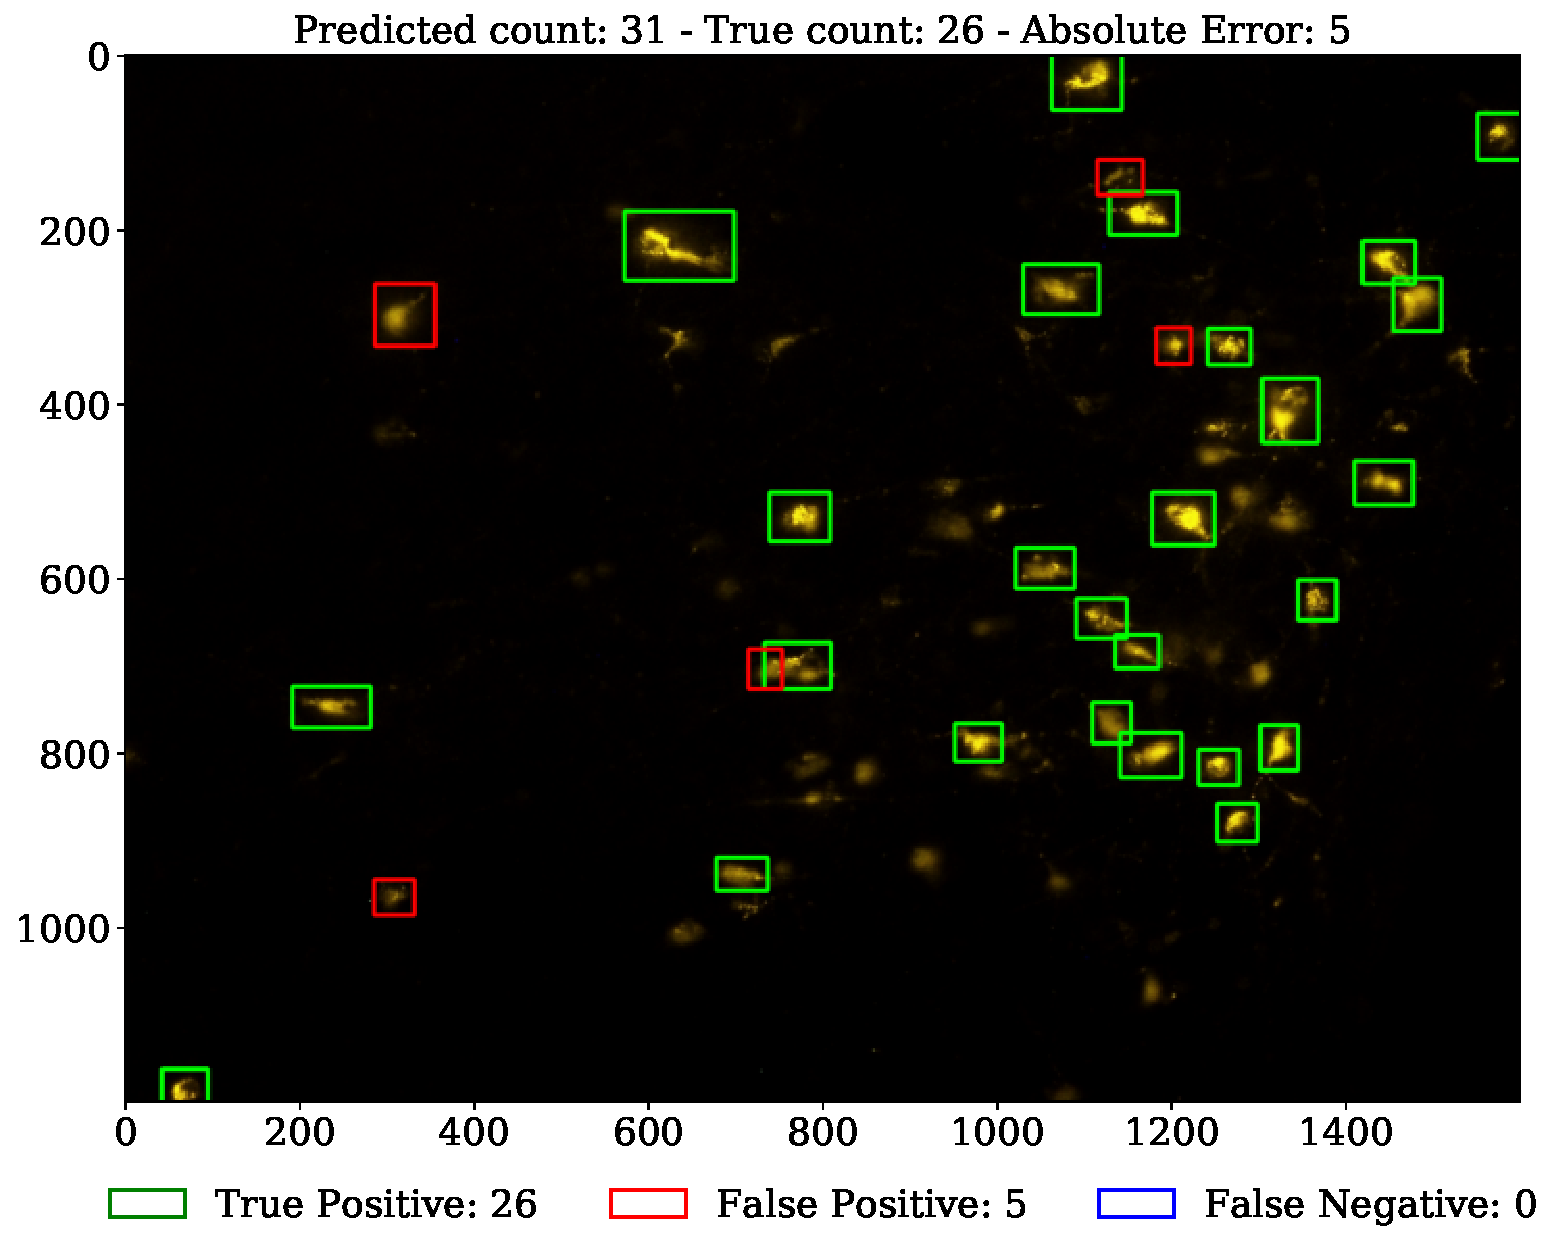
\includegraphics[width=\textwidth]{figures/140_results/pred_ResUnet:168.pdf}\label{fig:predictions:noAO}
% }
% \caption{\textbf{Results on test images}. 
% % Top row illustrates AO effect. 
% The c-ResUnet (no AO) correctly handles evident artifacts (\ref{fig:predictions:noAO}, top left corner), while the c-ResUnet fails with more problematic structures (\ref{fig:predictions:artifact}).
% % Bottom row highlights c-ResUnet predictive ability. 
% Notice how false positives (\ref{fig:predictions:false-positives}, red boxes) look like target cells. Likewise, the objects discarded (\ref{fig:predictions:false-negatives}, blue boxes) are similar to other stains that were not annotated.
% } 
% \label{fig:predictions}
% \end{figure}


% \begin{figure}[ht]\ContinuedFloat
% \centering
% \subfloat[]{
% 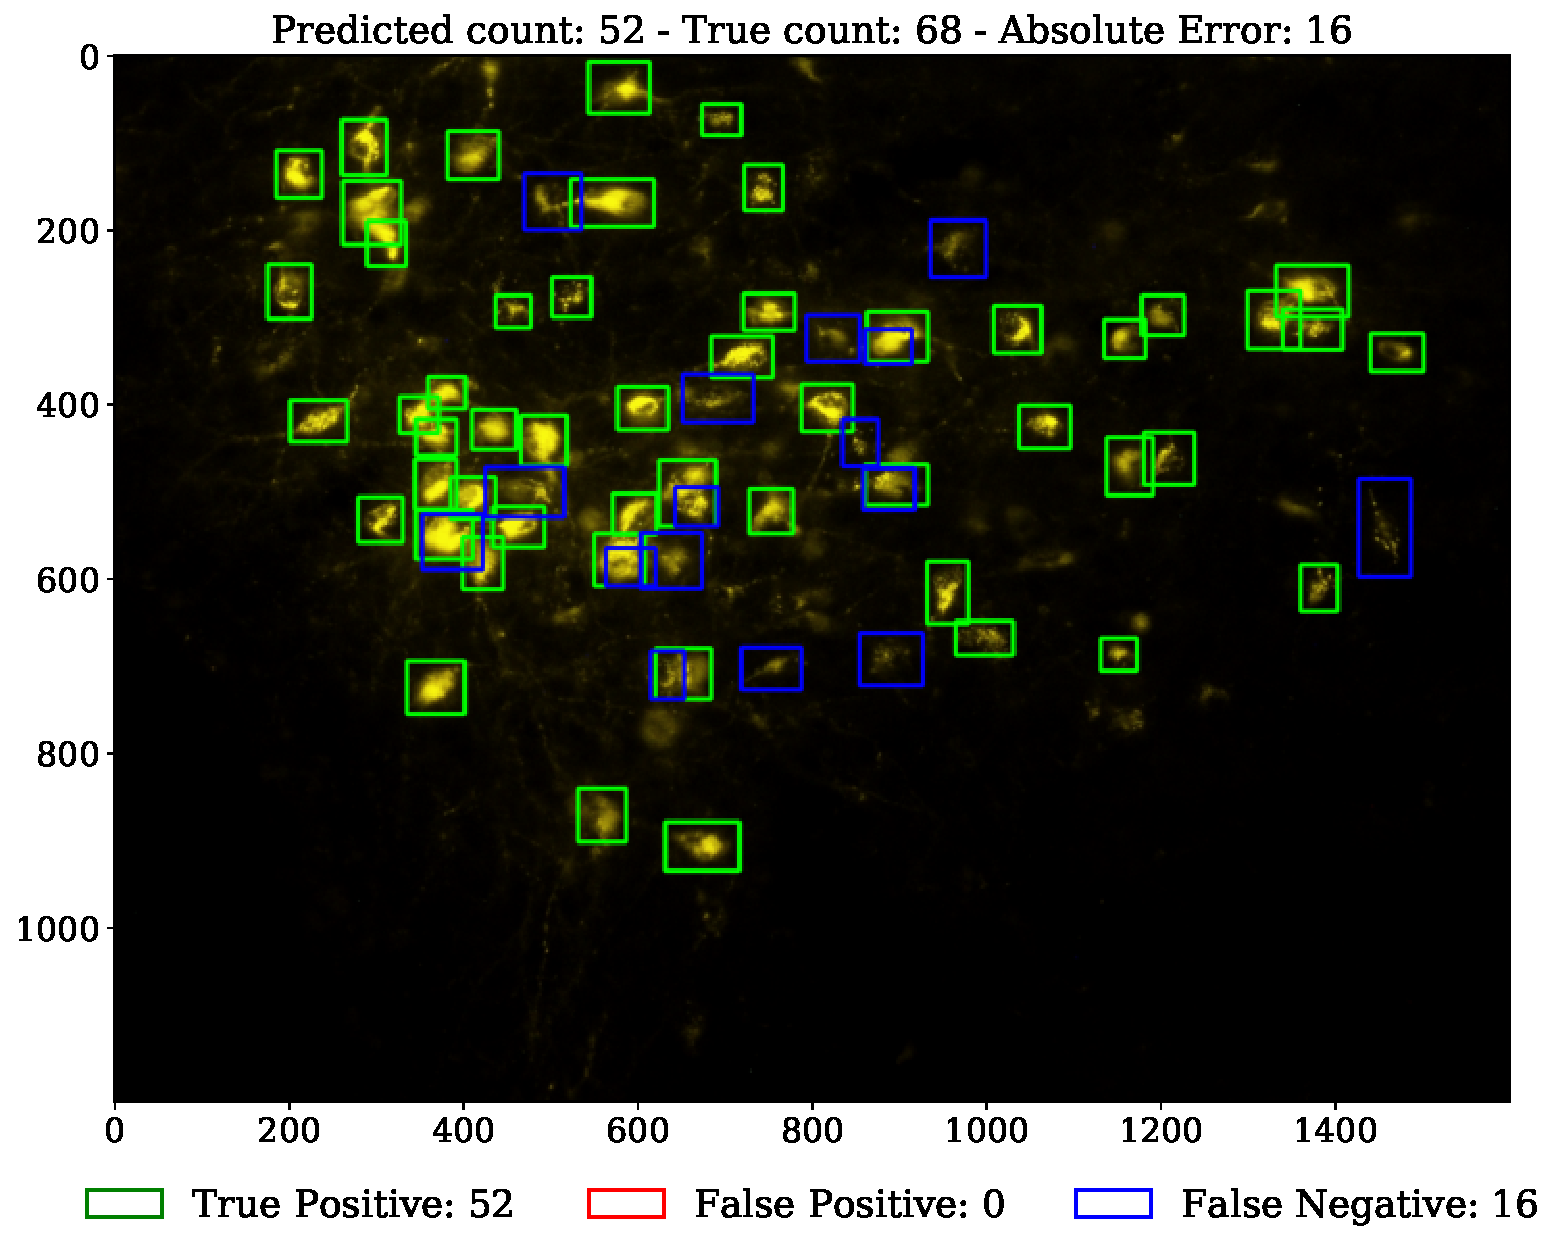
\includegraphics[width=\textwidth]{figures/140_results/pred_ResUnet:278.pdf}\label{fig:predictions:noAO}
% }
% \caption{\textbf{Results on test images}. 
% % Top row illustrates AO effect. 
% The c-ResUnet (no AO) correctly handles evident artifacts (\ref{fig:predictions:noAO}, top left corner), while the c-ResUnet fails with more problematic structures (\ref{fig:predictions:artifact}).
% % Bottom row highlights c-ResUnet predictive ability. 
% Notice how false positives (\ref{fig:predictions:false-positives}, red boxes) look like target cells. Likewise, the objects discarded (\ref{fig:predictions:false-negatives}, blue boxes) are similar to other stains that were not annotated.
% } 
% \label{fig:predictions}
% \end{figure}

% \clearpage
% \restoregeometry